\documentclass[aspectratio=169,xcolor=table]{beamer}
\usetheme{Madrid}

% ---------------------------------------------------------------
% Packages
% ---------------------------------------------------------------
\usepackage[utf8]{inputenc}
\usepackage{amsmath,amssymb}
\usepackage{booktabs}
\usepackage[round]{natbib}
\usepackage{array}
\usepackage{graphicx}
% figures/: static images; ../output/...: figures made by the repo's scripts, used as they are (compile from the repo)
\graphicspath{{figures/}{../output/hidden_states/norms/}{../output/hidden_states/within/}{../output/hidden_states/across/}
  {../output/hidden_states/surprisal/}{../output/time_space/}}
\usepackage{tikz}
\usetikzlibrary{arrows.meta,positioning,calc}
\usepackage{pgfplots}
\pgfplotsset{compat=1.16}

\setbeamertemplate{navigation symbols}{}

% ---------------------------------------------------------------
% Colours & helpers
% ---------------------------------------------------------------
\definecolor{mainblue}{RGB}{51,51,178}   % Madrid structure colour
\definecolor{human}{HTML}{1F77B4}
\definecolor{machine}{HTML}{FF7F0E}
\definecolor{good}{HTML}{2CA02C}
\definecolor{bad}{HTML}{D62728}
\definecolor{spgreen}{HTML}{1DB954}      % Spotify green

% Optional: switch the whole theme to a Spotify-green accent
% \usecolortheme[named=spgreen]{structure}

% Heat-map cell: 50 (red) -> 75 (yellow) -> 100 (green)
\newcommand{\hm}[1]{%
  \pgfmathtruncatemacro{\hmp}{max(0,min(100,(#1-50)*2))}%
  \ifnum\hmp<50
    \pgfmathtruncatemacro{\hmq}{2*\hmp}\edef\hmcol{yellow!\hmq!bad!45!white}%
  \else
    \pgfmathtruncatemacro{\hmq}{2*(\hmp-50)}\edef\hmcol{good!\hmq!yellow!45!white}%
  \fi
  \expandafter\cellcolor\expandafter{\hmcol}#1}

% Light-blue research-question block
\newenvironment{questionblock}[1]{%
  \setbeamercolor{block title}{fg=black, bg=human!30}%
  \setbeamercolor{block body}{fg=black, bg=human!10}%
  \begin{block}{#1}}{\end{block}}

% Light-grey approach box
\newenvironment{approachblock}[1]{%
  \setbeamercolor{block title}{fg=black, bg=black!15}%
  \setbeamercolor{block body}{fg=black, bg=black!5}%
  \begin{block}{#1}}{\end{block}}

% Light-green takeaway box
\setbeamercolor{takeaway}{fg=black, bg=spgreen!18}
\newenvironment{takeaway}{%
  \begin{beamercolorbox}[rounded=true, shadow=true, wd=\linewidth, sep=5pt]{takeaway}\small\ignorespaces}%
  {\end{beamercolorbox}}

% Spotify logo for table headers: place your logo file at figures/spotify_logo.png
\newcommand{\spotifylogo}{%
  \IfFileExists{figures/spotify_logo.png}%
    {\raisebox{-0.25\height}{
\includegraphics[height=1.3em]{spotify_logo.png}}}%
    {\textbf{Spotify}}}
% Hidden-state trajectory schematic (tokens x layers)
\newcommand{\trajschematic}{%
  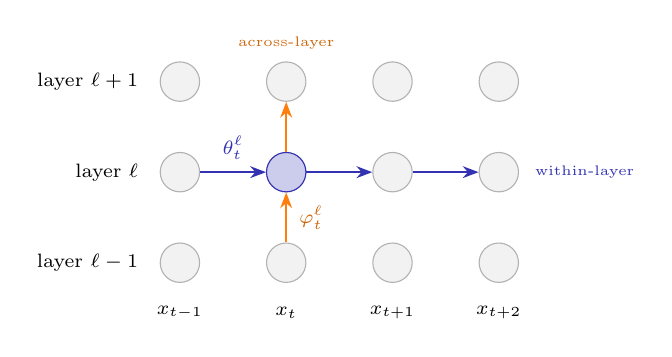
\begin{tikzpicture}[x=1.35cm, y=1.15cm,
      st/.style={circle, draw=gray!60, fill=gray!10, minimum size=5mm, inner sep=0pt}]
    \foreach \i in {0,...,3} \foreach \j in {0,1,2} \node[st] (n\i\j) at (\i,\j) {};
    \node[st, fill=mainblue!25, draw=mainblue] at (1,1) {};
    \foreach \j/\lab in {0/{\ell-1},1/{\ell},2/{\ell+1}}
      \node[font=\scriptsize, anchor=east] at (-0.3,\j) {layer $\lab$};
    \foreach \i/\lab in {0/{t-1},1/{t},2/{t+1},3/{t+2}}
      \node[font=\scriptsize] at (\i,-0.55) {$x_{\lab}$};
    \foreach \a/\b in {0/1,1/2,2/3}
      \draw[-{Stealth[length=2mm]}, thick, mainblue] (n\a1) -- (n\b1);
    \draw[-{Stealth[length=2mm]}, thick, machine] (n10) -- (n11);
    \draw[-{Stealth[length=2mm]}, thick, machine] (n11) -- (n12);
    \node[font=\scriptsize, text=mainblue, anchor=south] at (0.5,1.03) {$\theta^{\ell}_t$};
    \node[font=\scriptsize, text=machine!80!black, anchor=west] at (1.03,0.5) {$\varphi^{\ell}_t$};
    \node[font=\tiny, text=mainblue, anchor=west] at (3.25,1) {within-layer};
    \node[font=\tiny, text=machine!80!black, anchor=south] at (1,2.25) {across-layer};
  \end{tikzpicture}}

\newcommand{\placeholder}[1]{\textcolor{gray}{\textit{[Placeholder: #1]}}}
\newcommand{\source}[1]{\par\vfill{\tiny\textcolor{gray}{#1}}}

% ---------------------------------------------------------------
% Title
% ---------------------------------------------------------------
\title[Detecting AI-Generated Text]{Detecting AI-Generated Text from Within Language Models}
\subtitle{Spotify -- CP Research Meeting}
\author[G. Quaremba]{Gerrit Quaremba (KCL \& ICL)}
\institute[KCL \& ICL]{}
\date{November 16, 2026}

\AtBeginSection[]{
  \begin{frame}{Overview}
    \tableofcontents[currentsection]
  \end{frame}
}

\begin{document}

% ===============================================================
\begin{frame}
  \titlepage
\end{frame}

% ===============================================================
\begin{frame}{Overview}
  \begin{center}
    \textbf{Guiding question:} Can we reliably tell whether a text was written\\
    by a \textcolor{human}{\textbf{human}} or by an \textcolor{machine}{\textbf{LLM}}?
  \end{center}
  \vspace{0.2cm}
  \begin{columns}[T]
    \begin{column}{0.31\textwidth}
      \begin{block}{Paper 1 \,|\, TSM-Bench}
        \small Do detectors still work when people use LLMs the way they \emph{actually} do?\\[3pt]
        {\scriptsize\textcolor{gray}{ICLR 2026}}
      \end{block}
    \end{column}
    \begin{column}{0.31\textwidth}
      \begin{block}{Paper 2 \,|\, Linear Probing}
        \small Is ``machineness'' encoded as a simple direction \emph{inside} the LLM?\\[3pt]
        {\scriptsize\textcolor{gray}{EMNLP 2026}}
      \end{block}
    \end{column}
    \begin{column}{0.31\textwidth}
      \begin{block}{Paper 3 \,|\, JAS (Joint Angular Score)}
        \small Can hidden-state \emph{geometry} power a \emph{zero-shot} detector?\\[3pt]
        {\scriptsize\textcolor{gray}{Draft (ACL 2027 submission)}}
      \end{block}
    \end{column}
  \end{columns}
  \vspace{0.5cm}
  \begin{center}
    \small For each paper:\;
    \textbf{Motivation} $\rightarrow$ \textbf{Methodology} $\rightarrow$
    \textbf{Results} $\rightarrow$ \textbf{Takeaways for} \spotifylogo
  \end{center}
\end{frame}

% ===============================================================
\begin{frame}[label=glance]{Main Takeaways at a Glance}
  \begin{columns}[T]
    \begin{column}{0.31\textwidth}
      \begin{block}{Paper 1 \,|\, TSM-Bench}
        \small
        \textbf{Realistic AI use is much harder to detect.}
        \vspace{-2pt}\begin{enumerate}\footnotesize\setlength{\itemsep}{2pt}
          \item Detectors drop from \textbf{$>$93\%} to \textbf{47--73\%} on realistic AI edits.
          \item \textbf{Task-specific} training transfers -- generic training learns \textbf{shortcuts}.
        \end{enumerate}
      \end{block}
    \end{column}
    \begin{column}{0.31\textwidth}
      \begin{block}{Paper 2 \,|\, Linear Probing}
        \small
        \textbf{``Machineness'' is a direction inside the LLM.}
        \vspace{-2pt}\begin{enumerate}\footnotesize\setlength{\itemsep}{2pt}
          \item Human and AI text are \textbf{linearly separable} inside LLMs.
          \item Simple probes beat \textbf{16 detectors} (+11 AUC out-of-domain) with \textbf{$<$100 labels}.
        \end{enumerate}
      \end{block}
    \end{column}
    \begin{column}{0.31\textwidth}
      \begin{block}{Paper 3 \,|\, JAS (Joint Angular Score)}
        \small
        \textbf{AI text leaves a geometric fingerprint inside the LLM.}
        \vspace{-2pt}\begin{enumerate}\footnotesize\setlength{\itemsep}{2pt}
          \item AI tokens are \textbf{more aligned} and \textbf{rotate less} across layers.
          \item A \textbf{training-free} score beats \textbf{12 zero-shot detectors} (+8 AUC).
        \end{enumerate}
      \end{block}
    \end{column}
  \end{columns}
  \vspace{0.2cm}
  \begin{center}
    \small \textbf{Common thread:} realistic evaluation $\rightarrow$ robust, cheap detection
    from model internals $\rightarrow$ training-free detection from hidden-state geometry
  \end{center}
\end{frame}

% ###############################################################
\section[TSM-Bench]{Paper 1: TSM-Bench}
% ###############################################################

\begin{frame}{TSM-Bench \,|\, Motivation: Why Detect AI Text on Wikipedia?}
  \begin{columns}[c]
    \begin{column}{0.56\textwidth}
      \begin{itemize}
        \item Detection benchmarks generate AI text with \textbf{generic prompts}:
              \emph{``Write an article about machine learning.''}
        \item But editors use LLMs for \textbf{specific tasks}: summarising, extending
              a paragraph, rewriting a sentence\ldots
        \item Focus on \textbf{Wikipedia}, with tasks grounded in \textbf{interviews with editors}
              on their LLM use.
      \end{itemize}
    \end{column}
    \begin{column}{0.40\textwidth}
      \begin{questionblock}{Research question}
        Do detectors that look great on benchmarks still work when people use LLMs
        the way they \emph{actually} do?
      \end{questionblock}
    \end{column}
  \end{columns}
\end{frame}

% ---------------------------------------------------------------
\begin{frame}{TSM-Bench \,|\, Motivation: Generic vs.\ Task-Specific Generation}
  \begin{columns}[T]
    \begin{column}{0.48\textwidth}
      \begin{block}{Generic (prior benchmarks)}
        \small \emph{``Write a Wikipedia article about Machine Learning.''}
        \scriptsize -- unconstrained, no context.
      \end{block}
    \end{column}
    \begin{column}{0.48\textwidth}
      \begin{exampleblock}{Task-specific (real editing)}
        \small \emph{``Summarise this article to create the lead section\ldots\ \textless context\textgreater''}
        \scriptsize -- constrained task + context.
      \end{exampleblock}
    \end{column}
  \end{columns}
  \vspace{0.2cm}
  \centering
  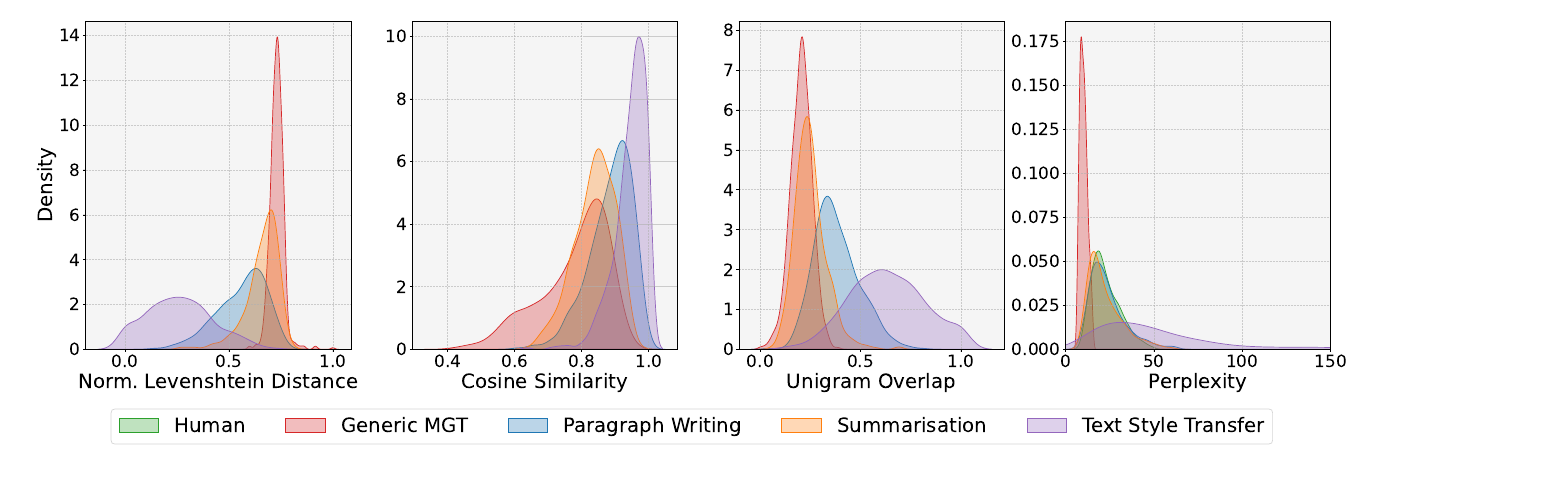
\includegraphics[width=0.86\textwidth]{tsm_fig1.png}\\[2pt]
  {\scriptsize Distance/overlap to the human reference and perplexity (English). Task-specific AI text
  sits much closer to human text $\Rightarrow$ more overlap, harder detection.}
\end{frame}

% ---------------------------------------------------------------
\begin{frame}{TSM-Bench \,|\, Methodology: Building the Benchmark}
  \centering
  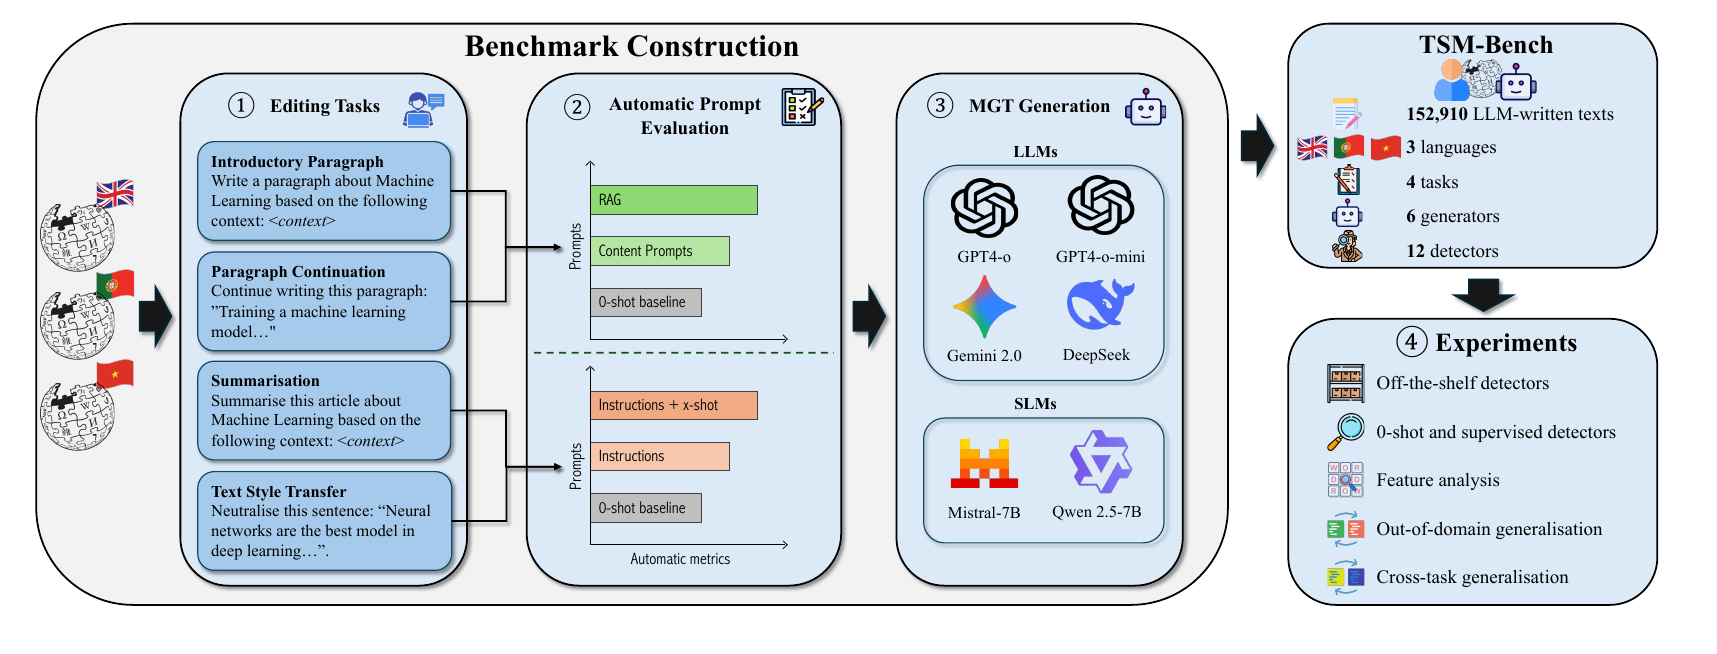
\includegraphics[width=0.92\textwidth]{tsm_fig2.png}\\[8pt]
  \raggedright\small
  \textbf{Key design choice:} the LLM gets \emph{context} (retrieved evidence, the article body, the biased
  sentence) -- just as a real editor would provide it.
\end{frame}

% ---------------------------------------------------------------


% ---------------------------------------------------------------
\begin{frame}{TSM-Bench \,|\, Result 1: Off-the-Shelf Detectors Collapse}
  \begin{columns}[c]
    \begin{column}{0.58\textwidth}
      \centering
      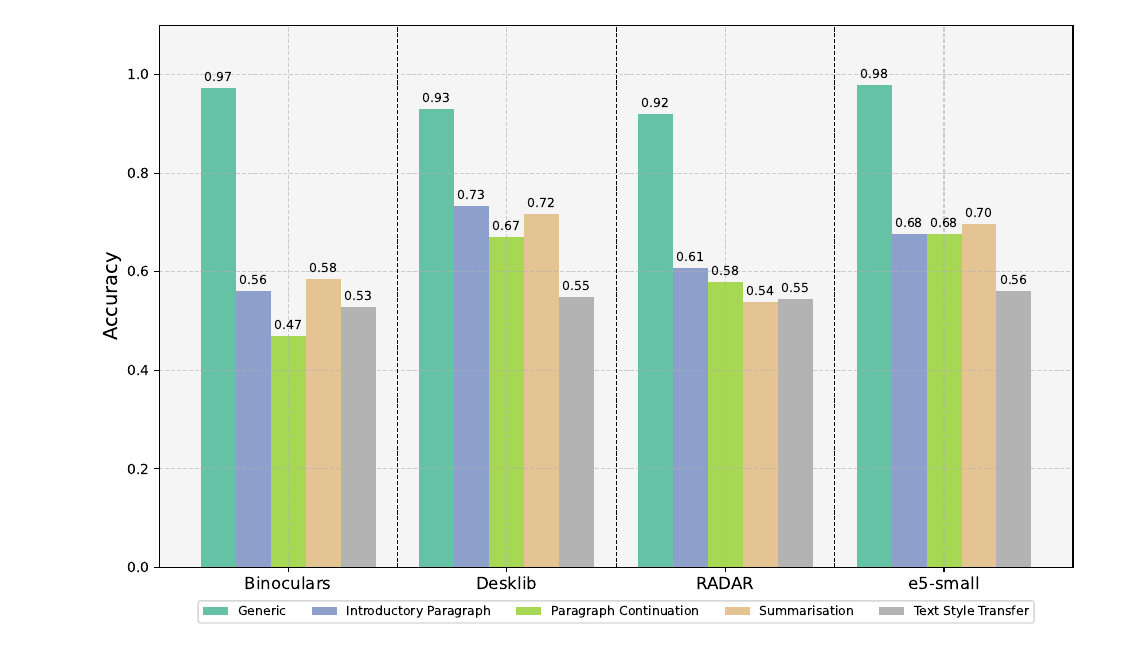
\includegraphics[width=\textwidth]{tsm_fig3.png}\\
      {\tiny Experiment 1: English, GPT-4o.}
    \end{column}
    \begin{column}{0.40\textwidth}
      \begin{itemize}
        \item On generic AI text: \textbf{$>$93\%} accuracy for all four detectors.
        \item On task-specific AI text: \textbf{47--73\%}.
        \item Even a top zero-shot method (Binoculars) falls close to chance.
      \end{itemize}
      \vspace{0.2cm}
      \begin{takeaway}
        Benchmarks built on generic prompts \textbf{overestimate} real-world performance.
      \end{takeaway}
    \end{column}
  \end{columns}
\end{frame}

% ---------------------------------------------------------------
\begin{frame}{TSM-Bench \,|\, Result 2: A Generalisation Asymmetry}
  \centering
  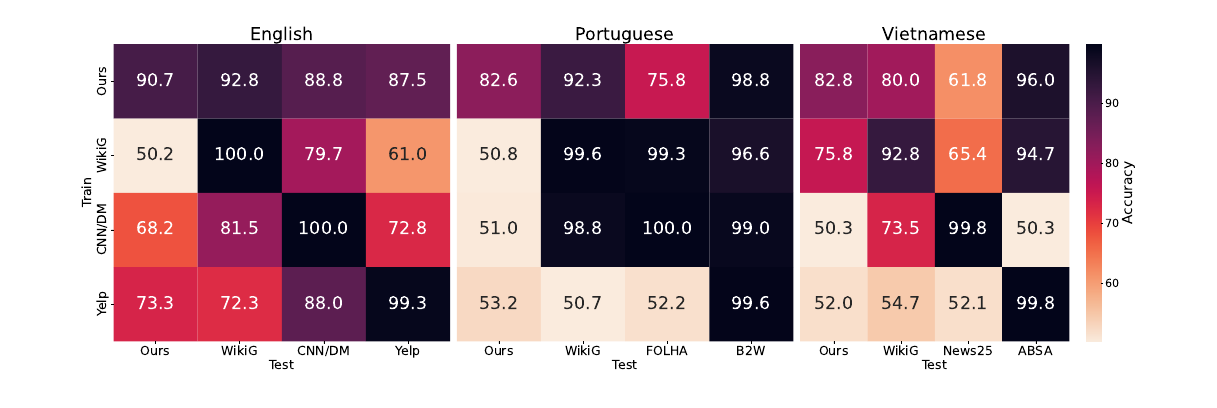
\includegraphics[width=0.76\textwidth]{tsm_fig4.png}\\
  {\tiny mDeBERTa, GPT-4o. ``Ours'' = task-specific; WikiG, news (CNN/DM, FOLHA, News25) and reviews (Yelp, B2W, ABSA) = generic AI text.}
  \vspace{0.1cm}
  \raggedright\footnotesize
  \begin{itemize}
    \item Trained on \textbf{task-specific} data $\Rightarrow$ generalises to generic AI text, even in other domains (first row).
    \item Trained on \textbf{generic} data $\Rightarrow$ fails on task-specific text, even within Wikipedia (first column, as low as 50\%).
  \end{itemize}
  \vspace{0.05cm}
  \begin{takeaway}
    Realistic, task-specific training data transfers to generic AI text -- but not the other way round.
  \end{takeaway}
\end{frame}

% ---------------------------------------------------------------
\begin{frame}{TSM-Bench \,|\, Result 3: Generic Training Teaches Shortcuts}
  \begin{columns}[c]
    \begin{column}{0.52\textwidth}
      \centering
      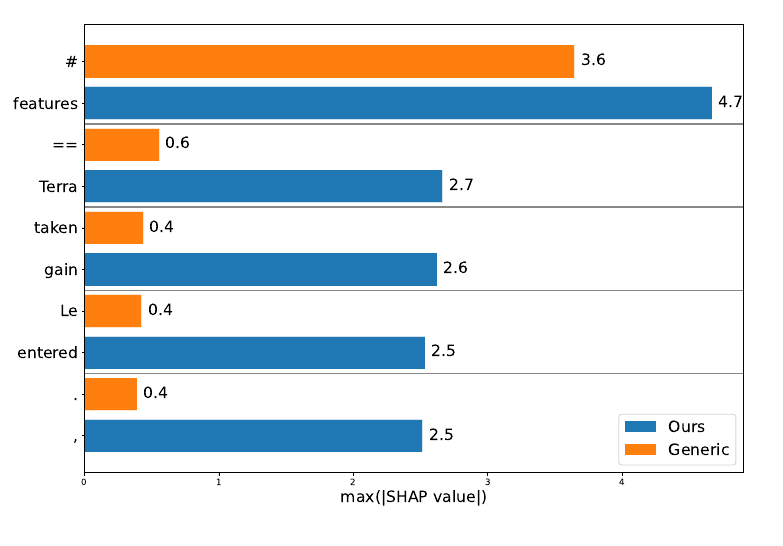
\includegraphics[width=\textwidth]{tsm_fig5.png}\\
      {\tiny Top SHAP tokens of mDeBERTa trained on generic vs.\ task-specific (``Ours'') English Wikipedia data.}
    \end{column}
    \begin{column}{0.45\textwidth}
      \small
      \begin{itemize}
        \item \textbf{Trained on generic data:} the strongest cues are \textbf{formatting artefacts}
              such as \texttt{\#} and \texttt{==} (markdown headers).
        \item \textbf{Trained on task-specific data:} weight shifts to content words that reflect
              \textbf{transferable} AI-writing patterns.
        \item This explains the asymmetry: generic detectors learn how AI text \emph{looks},
              not how it is \emph{written}.
      \end{itemize}
      \vspace{0.1cm}
      \begin{takeaway}
        Training on generic AI text makes detectors \textbf{overfit to superficial artefacts}
        that disappear in real-world use.
      \end{takeaway}
    \end{column}
  \end{columns}
\end{frame}

% ---------------------------------------------------------------
\begin{frame}{TSM-Bench \,|\, Main Takeaways}
  \footnotesize
  \renewcommand{\arraystretch}{1.5}
  \begin{tabular}{@{}>{\raggedright\arraybackslash}p{0.45\textwidth} >{\raggedright\arraybackslash}p{0.50\textwidth}@{}}
    \toprule
    \textbf{Takeaway} & \textbf{Why it matters for} \spotifylogo \\
    \midrule
    \textbf{1. Standard benchmarks overestimate detectors.}
    Realistic, task-specific AI text cuts accuracy by 10--40\%.
    & Evaluate detectors on content made the way creators really use LLMs
      (e.g.\ summarised show notes, polished episode descriptions, rewritten bios) --
      not on ``write an X'' samples. \\
    \textbf{2. Generalisation is asymmetric.}
    Task-specific training transfers to generic text, not vice versa; generic data
    teaches formatting shortcuts.
    & Invest in realistic, task-grounded training data. Detectors trained on
      generic synthetic text can look strong offline and fail in production. \\
    \bottomrule
  \end{tabular}
\end{frame}

% ###############################################################
\section[Linear Probing]{Paper 2: Linear Probing}
% ###############################################################

\begin{frame}{Linear Probing \,|\, Motivation}
  \begin{columns}[c]
    \begin{column}{0.56\textwidth}
      \textbf{The problem with current detectors}
      \begin{itemize}
        \item Supervised detectors top benchmarks, but \textbf{degrade out-of-domain}
              and need \textbf{large, diverse} training sets.
        \item Rewrite-based detectors add heavy compute overhead.
      \end{itemize}
      \vspace{0.2cm}
      \textbf{An opportunity: the Linear Representation Hypothesis}
      \begin{itemize}
        \item LLMs encode high-level concepts as \textbf{linear directions} in their
              activations -- e.g.\ truth, sentiment, political ideology.
      \end{itemize}
    \end{column}
    \begin{column}{0.40\textwidth}
      \begin{questionblock}{Research questions}
        \begin{enumerate}
          \item Are human and AI text \textbf{linearly separable} inside an LLM?
          \item If so, \textbf{why}?
          \item Can we exploit this for \textbf{better detection}?
        \end{enumerate}
      \end{questionblock}
      \vspace{0.1cm}
      {\small\emph{Idea: instead of reading the text, look at how the LLM represents it.}}
    \end{column}
  \end{columns}
\end{frame}

% ---------------------------------------------------------------
\begin{frame}{Linear Probing \,|\, Analysis: Human and AI Text Are Linearly Separable}
  \centering
  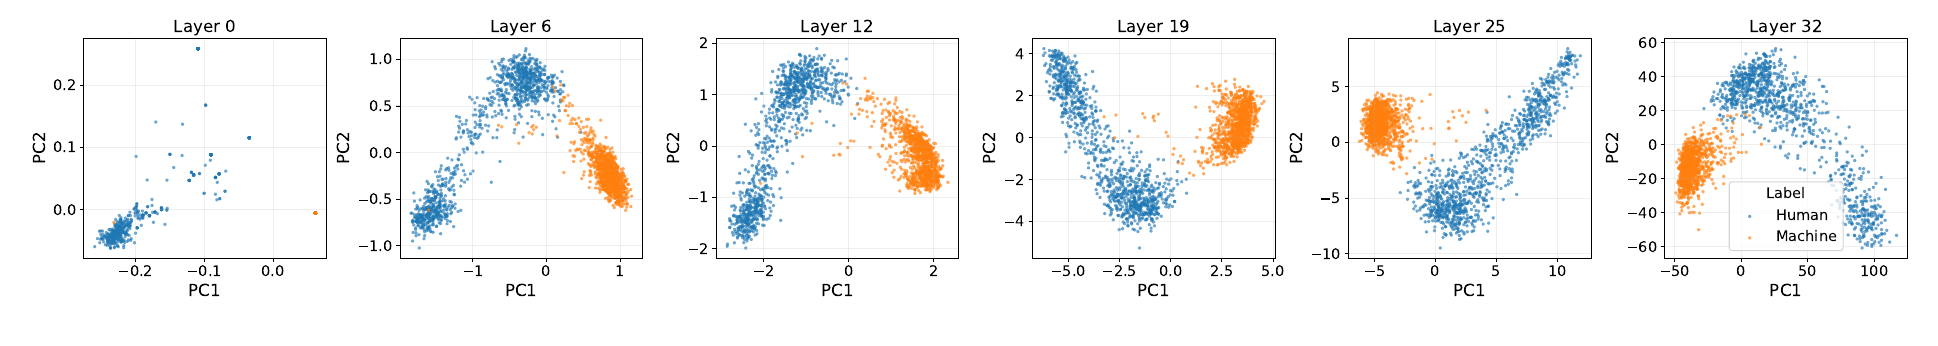
\includegraphics[width=0.92\textwidth]{lp_fig1.png}\\
  {\tiny Llama-3-8B hidden states of human (blue) and AI (orange) Wikipedia text, projected onto the first two principal components.}
  \vspace{0.15cm}
  \begin{columns}[c]
    \begin{column}{0.58\textwidth}
      \footnotesize
      \begin{itemize}
        \item Overlapping at layer 0, but \textbf{linearly separable from $\sim$layer 6} -- stable up to
              the last layer and across domains.
        \item \textbf{Is the boundary really linear?} Deeper MLP probes \textbf{lower} AUC
              $\Rightarrow$ extra non-linearity only hurts.
      \end{itemize}
      \vspace{0.1cm}
      \begin{takeaway}
        Inside the LLM, human and AI text are separated by a simple linear boundary.
      \end{takeaway}
    \end{column}
    \begin{column}{0.38\textwidth}
      \centering
      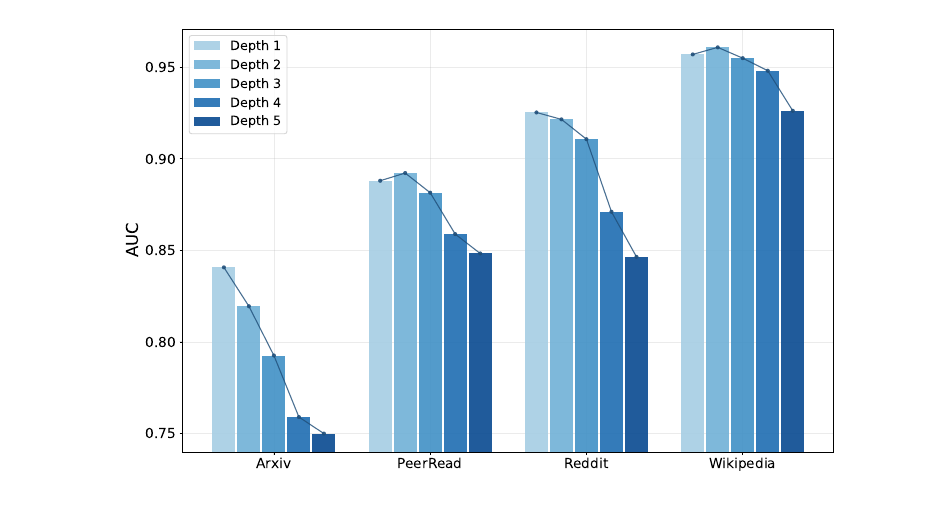
\includegraphics[width=\textwidth]{lp_fig2_id.png}\\
      {\tiny In-domain AUC of MLP probes with depth 1--5 (mid-layer).}
    \end{column}
  \end{columns}
\end{frame}

\begin{frame}{Linear Probing \,|\, Intuition: How a Linear Probe Separates Them}
  \begin{columns}[c]
    \begin{column}{0.45\textwidth}
      \centering
      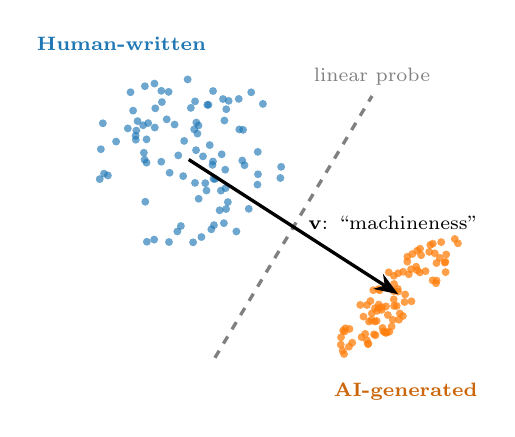
\begin{tikzpicture}[scale=0.95]
        \pgfmathsetseed{42}
        % human-written: wide, isotropic
        \foreach \i in {1,...,90}{
          \pgfmathsetmacro{\r}{1.25*sqrt(rnd)}
          \pgfmathsetmacro{\a}{360*rnd}
          \fill[human, opacity=0.65] ({-1.3+\r*cos(\a)},{0.9+\r*sin(\a)}) circle (1.5pt);
        }
        % machine-generated: compressed, anisotropic
        \foreach \i in {1,...,90}{
          \pgfmathsetmacro{\r}{sqrt(rnd)}
          \pgfmathsetmacro{\a}{360*rnd}
          \pgfmathsetmacro{\u}{1.1*\r*cos(\a)}
          \pgfmathsetmacro{\w}{0.30*\r*sin(\a)}
          \fill[machine, opacity=0.75] ({1.5+0.7071*(\u-\w)},{-0.9+0.7071*(\u+\w)}) circle (1.5pt);
        }
        \draw[dashed, very thick, gray] (-0.95,-1.75) -- (1.15,1.75)
          node[above, font=\scriptsize, text=gray] {linear probe};
        \draw[-{Stealth[length=3mm]}, very thick, black] (-1.3,0.9) -- (1.5,-0.9)
          node[pos=0.55, above right, font=\scriptsize, fill=white, fill opacity=0.85, text opacity=1, inner sep=1pt] {$\mathbf v$: ``machineness''};
        \node[font=\scriptsize\bfseries, text=human] at (-2.2,2.45) {Human-written};
        \node[font=\scriptsize\bfseries, text=machine!80!black] at (1.6,-2.2) {AI-generated};
      \end{tikzpicture}\\
      {\tiny Schematic illustration.}
    \end{column}
    \begin{column}{0.53\textwidth}
      \begin{itemize}
        \item A linear probe learns a \textbf{hyperplane} (dashed) between the two clouds.
        \item Its normal vector $\mathbf v$ is a \textbf{``machineness'' direction} in activation space.
        \item Projecting a new text onto $\mathbf v$ gives a \textbf{score}: the further along
              $\mathbf v$, the more ``machine-like''.
        \item Note the shapes: human text is \textbf{spread out}, AI text is
              \textbf{compressed} (next slide).
      \end{itemize}
    \end{column}
  \end{columns}
\end{frame}

% ---------------------------------------------------------------
\begin{frame}{Linear Probing \,|\, Analysis: Why? AI Text Is ``Compressed''}
  \centering
  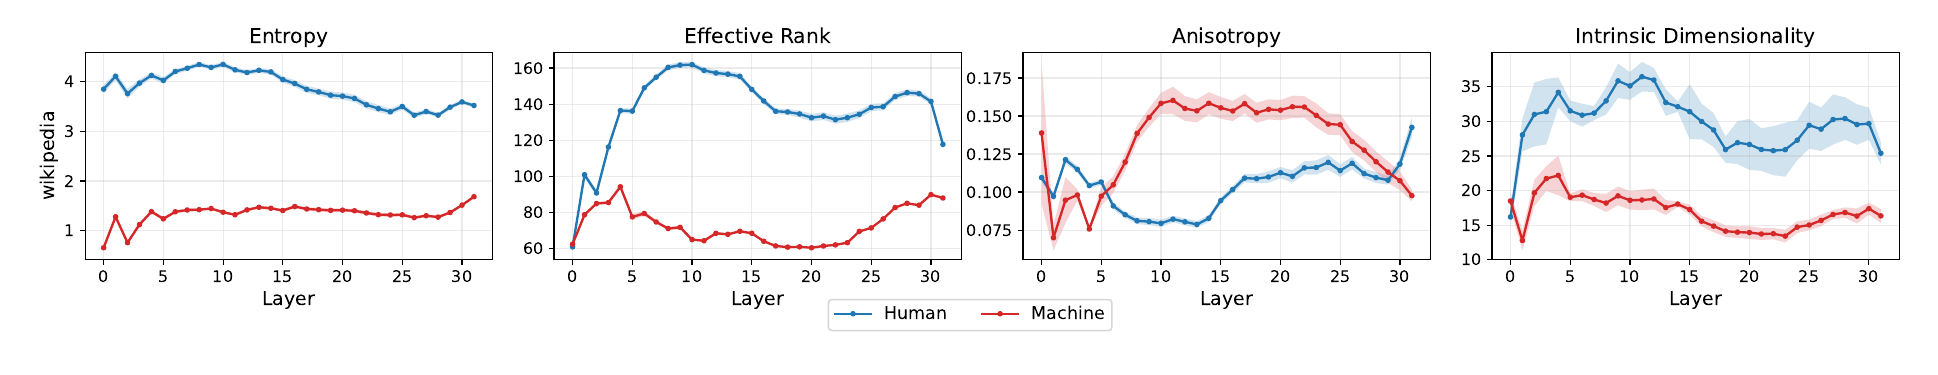
\includegraphics[width=\textwidth]{lp_fig3.png}\\
  {\tiny Representation-quality metrics per layer (Llama-3-8B, Wikipedia). Same pattern across 8 datasets.}
  \vspace{0.25cm}
  \begin{columns}[T]
    \begin{column}{0.52\textwidth}
      \small
      \begin{itemize}
        \item \textbf{Entropy, effective rank} (information content): \textcolor{bad}{lower} for AI text.
        \item \textbf{Anisotropy} (concentration on few directions): \textcolor{good}{higher} for AI text.
        \item \textbf{Intrinsic dimension} (manifold complexity): \textcolor{bad}{lower} for AI text.
      \end{itemize}
    \end{column}
    \begin{column}{0.44\textwidth}
      \begin{block}{Intuition}
        \small
        \textcolor{human}{\textbf{Human text}} activates a rich, diverse set of features.
        \textcolor{machine!80!black}{\textbf{AI text}} collapses into a narrow, low-dimensional
        subspace $\Rightarrow$ one hyperplane suffices.
      \end{block}
    \end{column}
  \end{columns}
\end{frame}

% ---------------------------------------------------------------
\begin{frame}{Linear Probing \,|\, Methodology: MGT Probes}
  \centering
  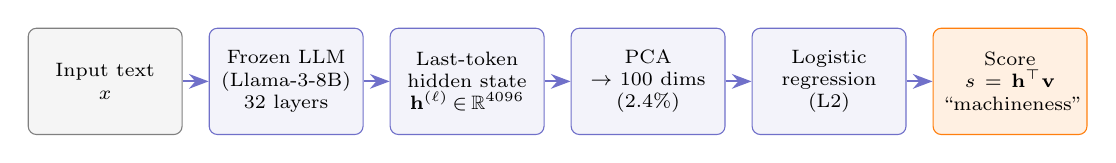
\begin{tikzpicture}[
      box/.style={draw=mainblue!70, fill=mainblue!6, rounded corners=3pt, align=center,
                  font=\scriptsize, minimum height=1.35cm, text width=1.72cm},
      arr/.style={-{Stealth[length=2.5mm]}, thick, mainblue!70}]
    \node[box, fill=gray!8, draw=gray] (x) {Input text\\$x$};
    \node[box, right=0.33cm of x] (llm) {Frozen LLM\\(Llama-3-8B)\\32 layers};
    \node[box, right=0.33cm of llm] (h) {Last-token\\hidden state\\$\mathbf h^{(\ell)}\!\in\!\mathbb R^{4096}$};
    \node[box, right=0.33cm of h] (pca) {PCA\\$\rightarrow$ 100 dims\\(2.4\%)};
    \node[box, right=0.33cm of pca] (lr) {Logistic\\regression\\(L2)};
    \node[box, right=0.33cm of lr, fill=machine!12, draw=machine] (s) {Score\\$s=\mathbf h^{\top}\mathbf v$\\``machineness''};
    \foreach \a/\b in {x/llm, llm/h, h/pca, pca/lr, lr/s} \draw[arr] (\a) -- (\b);
  \end{tikzpicture}
  \vspace{0.35cm}

  \begin{columns}[T]
    \begin{column}{0.47\textwidth}
      \begin{block}{LLP -- Layer-averaged Linear Probe}
        \small One probe per layer, average the projection scores:
        \[ s_{\text{LLP}}(x) = \tfrac{1}{L}\textstyle\sum_{\ell=1}^{L} {\mathbf h^{(\ell)}}^{\!\top}\mathbf v^{(\ell)} \]
      \end{block}
    \end{column}
    \begin{column}{0.47\textwidth}
      \begin{block}{CLP -- Concatenated-layer Linear Probe}
        \small One probe on all layers at once, learning which layers matter:
        \[ \mathbf h^{\text{concat}} = [\mathbf h^{(1)};\dots;\mathbf h^{(L)}] \in \mathbb R^{L\times 100} \]
      \end{block}
    \end{column}
  \end{columns}
  \vspace{0.15cm}
  {\footnotesize $\mathbf v = \mathbf w/\lVert\mathbf w\rVert$ is the normalised probe weight.
  Training incl.\ feature extraction: \textbf{1--3 minutes} on one A100.}
\end{frame}

% ---------------------------------------------------------------
\begin{frame}{Linear Probing \,|\, Result 1: In-Domain Detection}
  \centering
  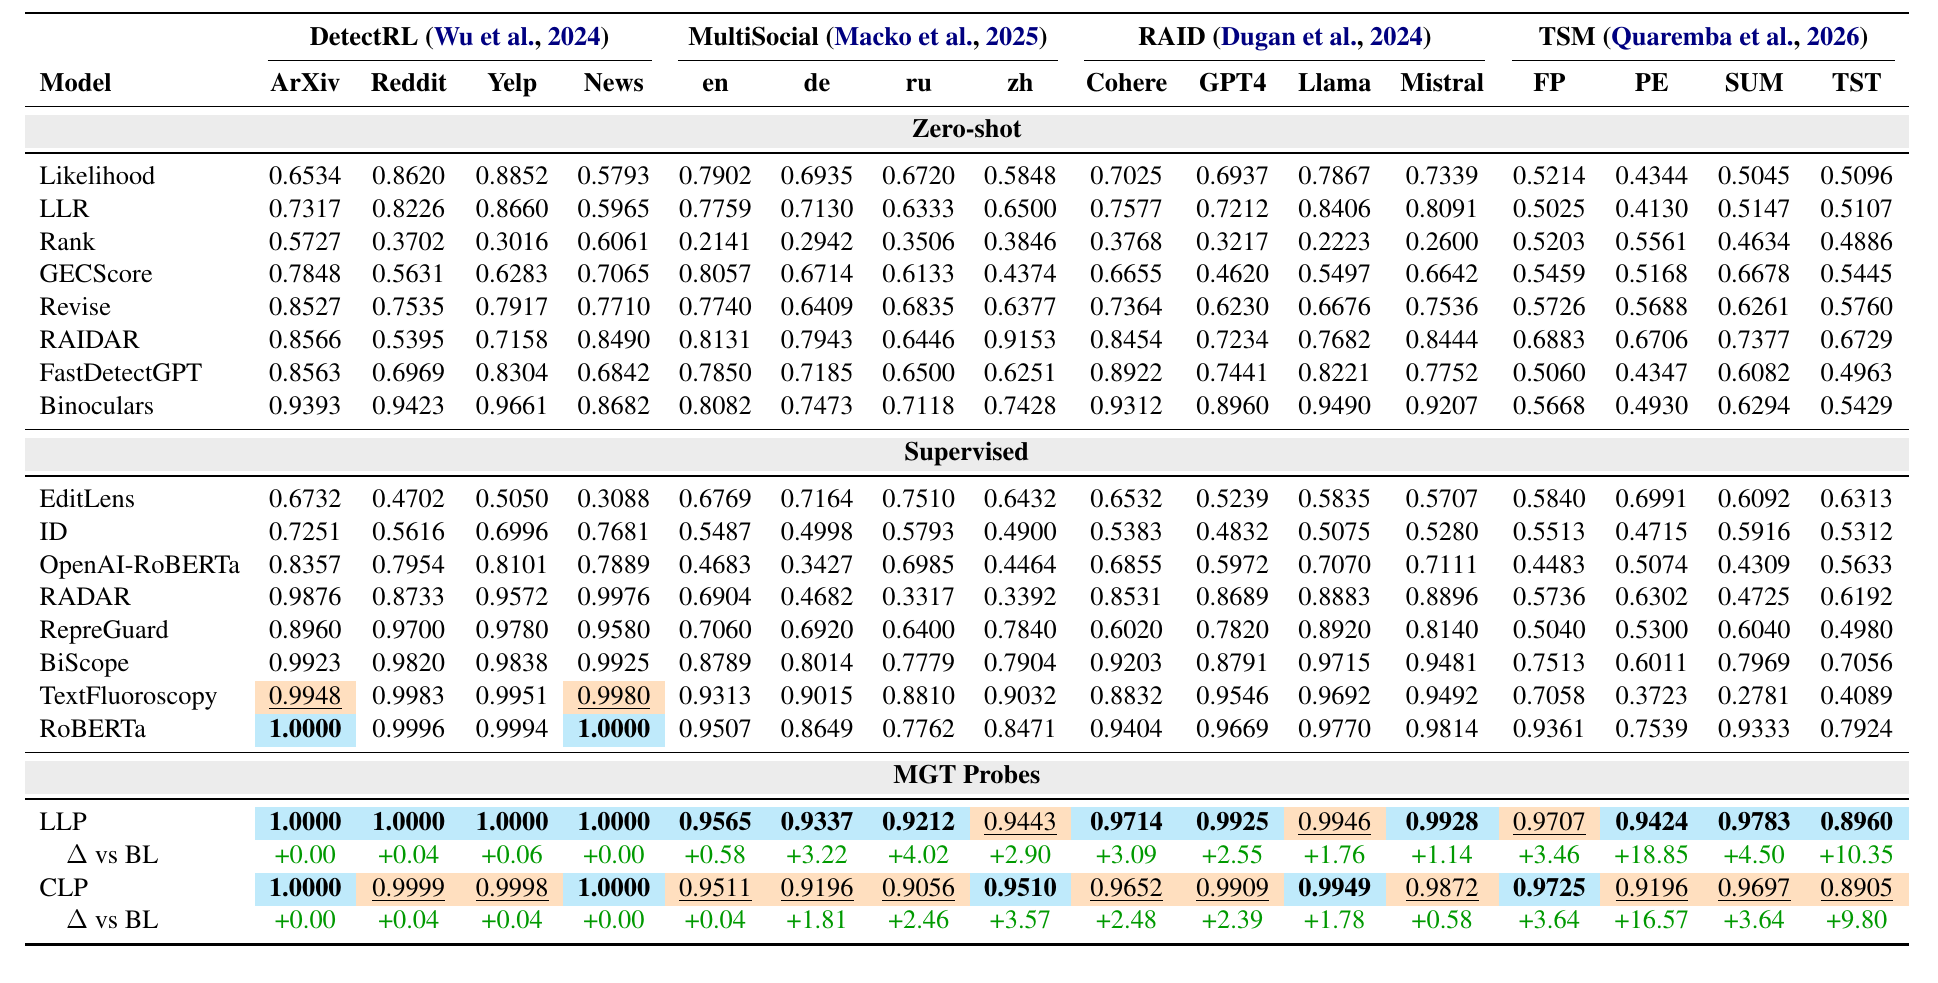
\includegraphics[width=0.74\textwidth]{lp_tab1.png}\\[4pt]
  \begin{takeaway}
    Linear probes beat all 16 detectors in every in-domain setting (+0.04 to +18.85 AUC), with the
    largest gains on the hardest benchmark, TSM.
  \end{takeaway}
\end{frame}

\begin{frame}{Linear Probing \,|\, Result 2: Out-of-Domain Detection}
  \centering
  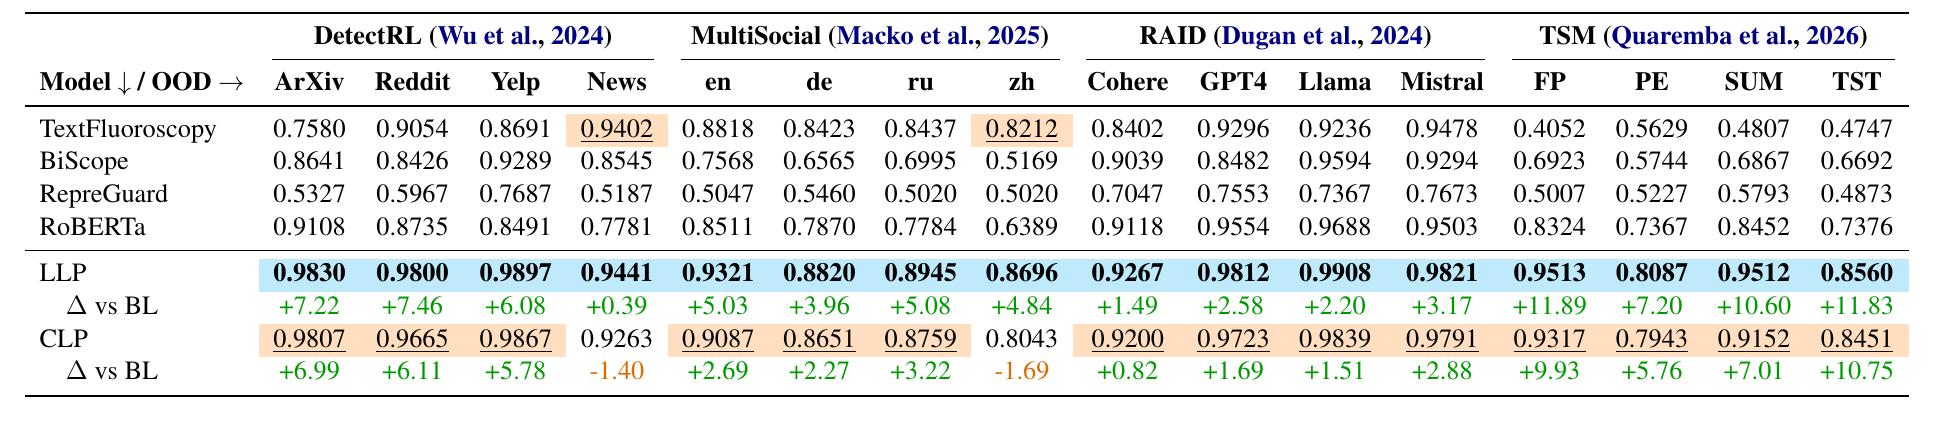
\includegraphics[width=0.95\textwidth]{lp_tab2.png}\\
  {\tiny Each column: mean AUC when training on the other three subsets of the same benchmark and testing on this one.}
  \vspace{0.15cm}
  \raggedright\footnotesize
  \begin{itemize}
    \item Probes \textbf{transfer best}: +0.4 to +11.9 AUC over the strongest supervised detectors.
    \item \textbf{Cross-lingual} transfer works even between distant languages (e.g.\ ru $\rightarrow$ zh).
    \item Largest gains \textbf{across tasks} (TSM: +5.8 to +11.9).
  \end{itemize}
  \vspace{0.1cm}
  \begin{takeaway}
    Probes generalise across domains, languages and tasks -- where supervised detectors fail.
  \end{takeaway}
\end{frame}

% ---------------------------------------------------------------
\begin{frame}{Linear Probing \,|\, Result 3: Why Do Probes Work So Well?}
  \begin{columns}[T]
    \begin{column}{0.31\textwidth}
      \centering\textbf{\small A shared direction}\\[3pt]
      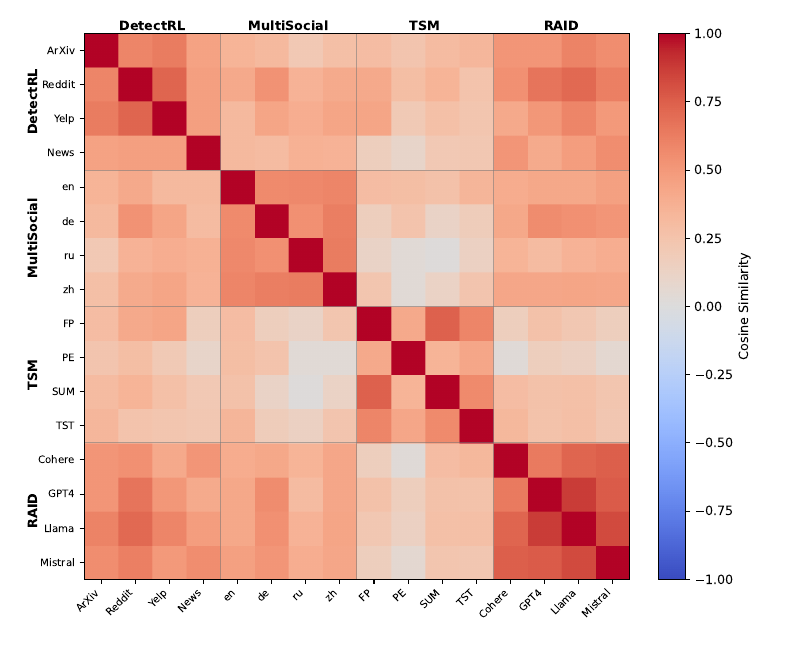
\includegraphics[width=0.72\textwidth]{lp_fig4.png}\\[3pt]
      \raggedright\scriptsize Probe vectors from 16 datasets are highly aligned within, and moderately
      across, benchmarks $\Rightarrow$ explains OOD transfer.
    \end{column}
    \begin{column}{0.34\textwidth}
      \centering\textbf{\small Sample-efficient}\\[3pt]
      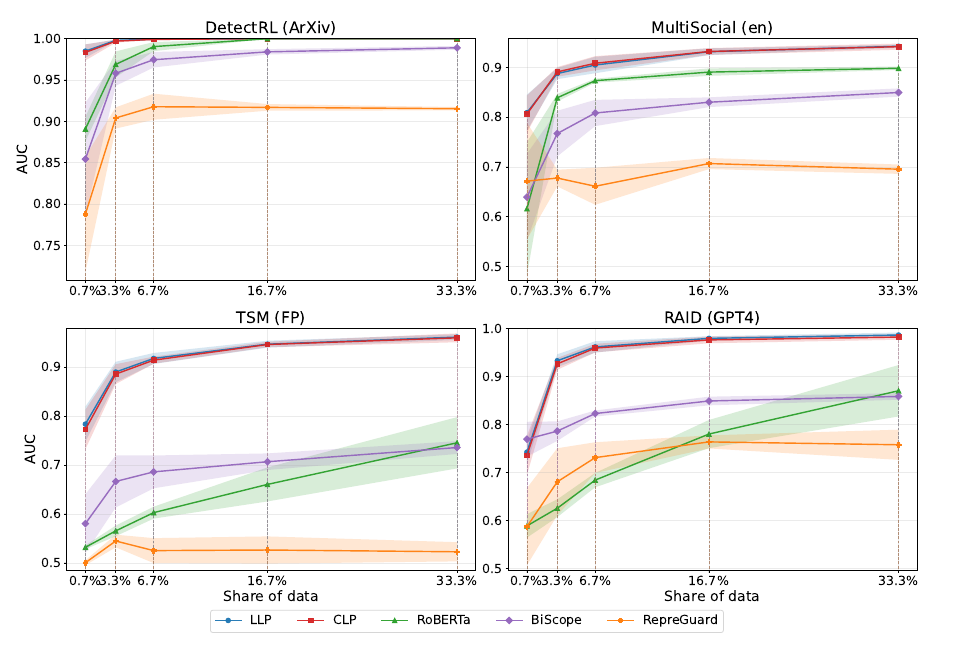
\includegraphics[width=0.88\textwidth]{lp_fig5.png}\\[3pt]
      \raggedright\scriptsize Near-peak AUC with only \textbf{10--100 labelled examples}, with lower
      variance than RoBERTa or RepreGuard.
    \end{column}
    \begin{column}{0.33\textwidth}
      \centering\textbf{\small A continuous score}\\[3pt]
      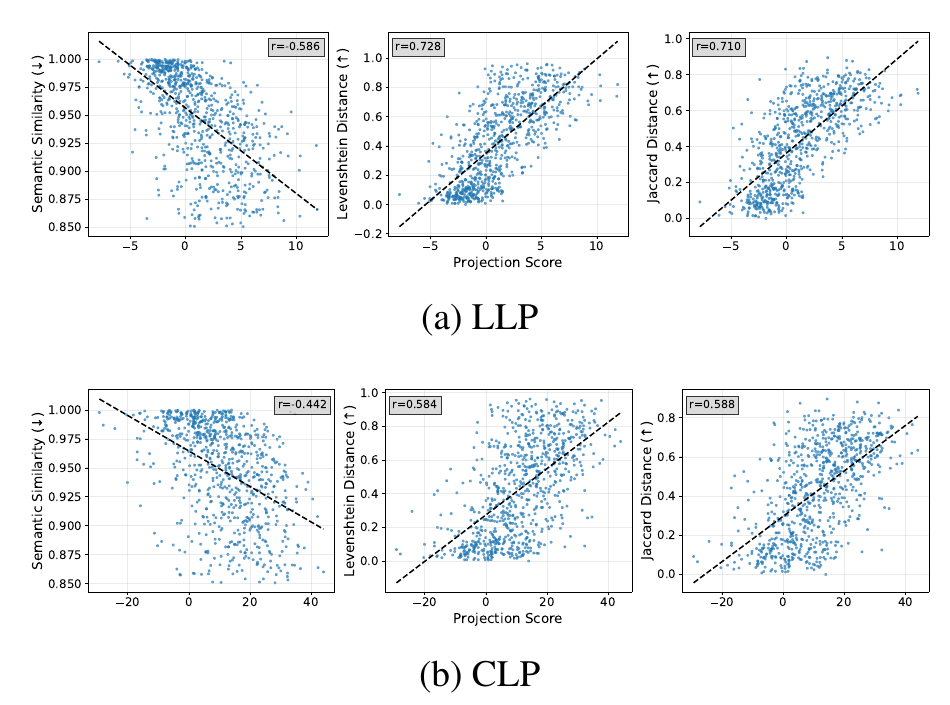
\includegraphics[width=0.84\textwidth]{lp_fig6.png}\\[3pt]
      \raggedright\scriptsize The score tracks \emph{how much} a text was AI-edited; 3-way
      classification: \textbf{85\%} vs.\ 65\% (RoBERTa).
    \end{column}
  \end{columns}
  \vspace{0.15cm}
  \begin{takeaway}
    A shared ``machineness'' direction makes probes transferable, label-efficient and able to grade
    the degree of AI editing.
  \end{takeaway}
\end{frame}

% ---------------------------------------------------------------
\begin{frame}{Linear Probing \,|\, Main Takeaways}
  \small
  \renewcommand{\arraystretch}{1.5}
  \begin{tabular}{@{}>{\raggedright\arraybackslash}p{0.45\textwidth} >{\raggedright\arraybackslash}p{0.50\textwidth}@{}}
    \toprule
    \textbf{Takeaway} & \textbf{Why it matters for} \spotifylogo \\
    \midrule
    \textbf{1. ``Machineness'' is a linear, low-dimensional direction}
    inside LLMs -- AI text is compressed and anisotropic.
    & A cheap add-on to LLM forward passes: 100-dim features + logistic regression,
      trained in minutes -- no large detector to fine-tune or serve. \\
    \textbf{2. Simple probes beat 16 detectors}, especially out-of-domain (+11 AUC)
    and across languages.
    & One model that transfers across markets, languages and new content types,
      instead of retraining per language or surface. \\
    \textbf{3. Few labels, graded output.} 10--100 examples suffice, and the score reflects
    the \emph{degree} of AI editing.
    & Only small labelled datasets are needed for new surfaces, and a continuous
      ``AI-assistance'' score can support nuanced policies (disclosure, review triage). \\
    \bottomrule
  \end{tabular}
  \vspace{0.15cm}

  {\scriptsize \textbf{Caveat:} requires access to hidden states (open-weight models);
  universality of the direction is not yet established.}
\end{frame}

% ###############################################################
\section[JAS]{Paper 3: JAS (Joint Angular Score)}
% ###############################################################

\begin{frame}{JAS \,|\, Motivation}
  \begin{columns}[c]
    \begin{column}{0.56\textwidth}
      \begin{itemize}
        \item \textbf{Supervised detectors} are the most accurate, but need large, diverse training
              data and generalise poorly out-of-domain (Paper 1).
        \item \textbf{Zero-shot detectors} need no training data and are more consistent across
              domains -- but are less accurate.
        \item \textbf{Representation-based detectors} are data-efficient and robust (Paper 2) --
              but still supervised.
      \end{itemize}
    \end{column}
    \begin{column}{0.40\textwidth}
      \begin{questionblock}{Research question}
        How can we design a \textbf{zero-shot}, \textbf{representation-based} AI text detector?
      \end{questionblock}
      \vspace{0.1cm}
      \begin{approachblock}{Approach}
        \small
        \begin{enumerate}
          \item Do human and AI hidden states differ \emph{per text} -- and how?
          \item Can these differences power zero-shot detection?
        \end{enumerate}
      \end{approachblock}
    \end{column}
  \end{columns}
\end{frame}

% ---------------------------------------------------------------
\begin{frame}{JAS \,|\, Analysis: Texts as Trajectories Through Hidden-State Space}
  \begin{columns}[c]
    \begin{column}{0.44\textwidth}
      \centering
      \scalebox{0.9}{\trajschematic}\\[4pt]
      {\tiny Hidden states of Llama-3.1-8B (32 layers).}
    \end{column}
    \begin{column}{0.54\textwidth}
      \small
      \begin{itemize}
        \item Feed a text through a surrogate LM -- we use \textbf{Llama-3.1-8B} -- and treat its hidden states as a
              \textbf{trajectory}, an idea borrowed from research on reasoning and language processing
              {\footnotesize\citep{wang2025latent,hosseini2023large}}.
        \item \textcolor{mainblue}{\textbf{Within-layer}}: how representations move from token to
              token at a fixed layer $\ell$ $\rightarrow$ angle $\theta^{\ell}_t$.
        \item \textcolor{machine!80!black}{\textbf{Across-layer}}: how one token's representation
              changes from layer to layer $\rightarrow$ angle $\varphi^{\ell}_t$.
        \item Both views are measured by \textbf{angular deviation}: the angle between consecutive hidden states.
      \end{itemize}
    \end{column}
  \end{columns}
\end{frame}

% ---------------------------------------------------------------
\begin{frame}{JAS \,|\, Analysis: The Two Trajectories, Formally}
  \small
  Let $x=(x_1,\dots,x_T)$ be a text and $\mathbf h_t^{\ell}\in\mathbb R^d$ the hidden state of token $x_t$ at layer
  $\ell\in\{0,\dots,L\}$ of the surrogate LM ($\ell=0$: embeddings). Angles between hidden states:
  \[
    \angle(\mathbf a,\mathbf b)=\arccos\frac{\langle\mathbf a,\mathbf b\rangle}{\lVert\mathbf a\rVert\,\lVert\mathbf b\rVert}
  \]
  \vspace{-4pt}
  \begin{columns}[T]
    \begin{column}{0.48\textwidth}
      \textcolor{mainblue}{\textbf{Within-layer trajectory}} -- fix a layer $\ell$, move along the text:
      \[
        \mathcal W^{\ell}(x)=\big(\mathbf h_1^{\ell},\,\mathbf h_2^{\ell},\,\dots,\,\mathbf h_T^{\ell}\big)
      \]
      step angle between consecutive tokens:
      \[
        \theta_t^{\ell}=\angle\big(\mathbf h_{t-1}^{\ell},\,\mathbf h_t^{\ell}\big),\quad t=2,\dots,T
      \]
    \end{column}
    \begin{column}{0.48\textwidth}
      \textcolor{machine!80!black}{\textbf{Across-layer trajectory}} -- fix a token $x_t$, move through the layers:
      \[
        \mathcal A_t(x)=\big(\mathbf h_t^{0},\,\mathbf h_t^{1},\,\dots,\,\mathbf h_t^{L}\big)
      \]
      step angle between consecutive layers:
      \[
        \varphi_t^{\ell}=\angle\big(\mathbf h_t^{\ell-1},\,\mathbf h_t^{\ell}\big),\quad \ell=1,\dots,L
      \]
    \end{column}
  \end{columns}
  \vspace{2pt}
  \begin{takeaway}
    A text gives one within-layer trajectory per layer and one across-layer trajectory per token; small angles mean
    a smooth, slowly turning path.
  \end{takeaway}
\end{frame}

% ---------------------------------------------------------------
\begin{frame}{JAS \,|\, Analysis}
  \vfill
  \centering
  {\Large Do the two trajectories differ \textbf{systematically}\\[4pt] between human and AI text?\\[10pt]
  And if so, \textbf{how}?}
  \vfill
\end{frame}

% ---------------------------------------------------------------
\begin{frame}{JAS \,|\, Analysis: Within-Layer -- AI Tokens Are Closer}
  \centering
  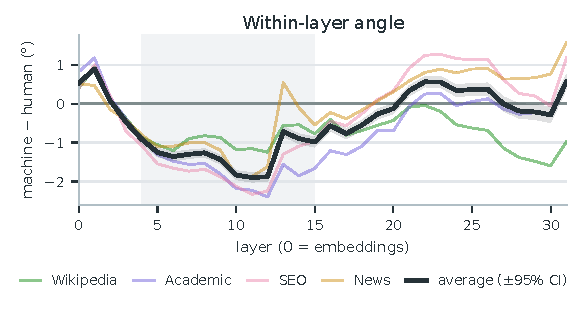
\includegraphics[width=\textwidth,height=3.65cm,keepaspectratio]{f_within_talk_A.pdf}\\
  {\tiny Machine $-$ human gap per layer, Llama-3.1-8B, four DetectRL-X domains (300 texts each); grey band: layers 4--15.}
  \vspace{0.05cm}
  \raggedright\footnotesize
  \begin{itemize}\setlength{\itemsep}{1pt}
    \item In layers 4--15, adjacent AI tokens are \textbf{1--1.7$^\circ$ closer} on average (up to 2.4$^\circ$), in
          \textbf{all four domains}.
    \item Outside this band the gap is small and changes sign across domains.
  \end{itemize}
  \begin{takeaway}
    In early-to-middle layers, AI tokens are closer to their neighbours. \textbf{Why?}
  \end{takeaway}
\end{frame}

% ---------------------------------------------------------------
\begin{frame}{JAS \,|\, Analysis: Within-Layer -- Why Are AI Neighbours Closer?}
  \centering
  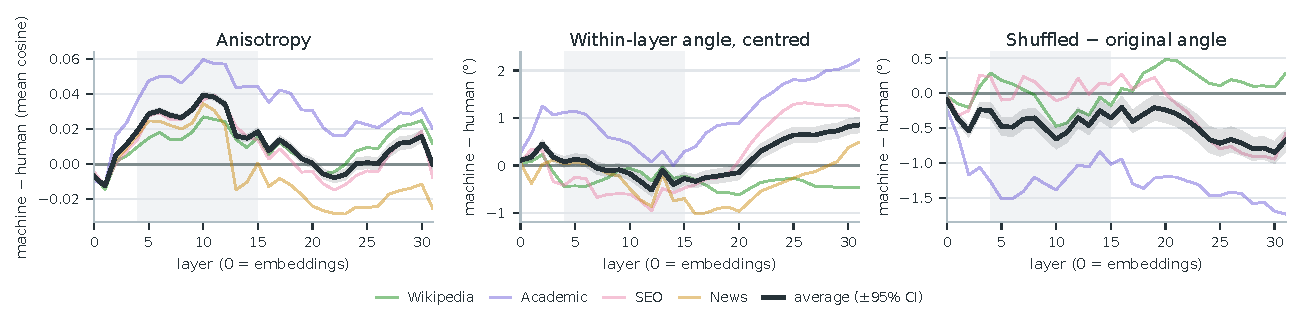
\includegraphics[width=\textwidth,height=3.1cm,keepaspectratio]{f_within_talk_B.pdf}\\
  {\tiny Machine $-$ human gap per layer, Llama-3.1-8B. Centred: each text's mean hidden state subtracted. Right:
  random token pairs minus adjacent pairs (no News yet).}
  \vspace{0.05cm}
  \raggedright\footnotesize
  \begin{itemize}\setlength{\itemsep}{0pt}
    \item \textbf{Anisotropy:} AI tokens share one direction more strongly (+0.02 to +0.05, on $\approx$0.24).
    \item \textbf{Centred:} removing it shrinks the gap to about a third ($-$0.3 to $-$0.6$^\circ$).
    \item \textbf{Random pairs $-$ neighbours:} word order adds no AI advantage ($\approx$0, or less local).
  \end{itemize}
  \begin{takeaway}
    \textbf{Finding 1:} within-layer angles are smaller because machine text is more anisotropic than human text in
    early-to-middle layers.
  \end{takeaway}
\end{frame}

% ---------------------------------------------------------------
\begin{frame}{JAS \,|\, Intuition: AI Text Lives in a Narrower Cone}
  \begin{columns}[T]
    \begin{column}{0.48\textwidth}
      \centering
      \textbf{\textcolor{human}{Human-written text}}\\[4pt]
      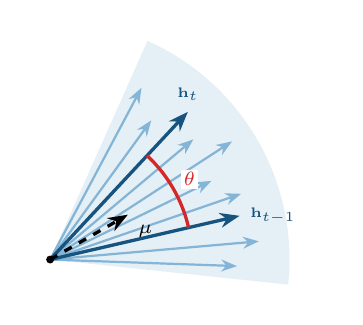
\begin{tikzpicture}[scale=0.95]
        \useasboundingbox (-0.3,-0.5) rectangle (3.8,3.1);
        \fill[human!12] (0,0) -- (-6:3.2) arc[start angle=-6, end angle=66, radius=3.2] -- cycle;
        \foreach \a/\r in {-2/2.5, 5/2.8, 19/2.7, 26/2.4, 33/2.9, 40/2.5, 54/2.3, 62/2.6}
          \draw[-{Stealth[length=2mm]}, human!55, thick] (0,0) -- (\a:\r);
        \draw[-{Stealth[length=2.5mm]}, human!70!black, very thick] (0,0) -- (13:2.6) node[right, font=\tiny] {$\mathbf h_{t-1}$};
        \draw[-{Stealth[length=2.5mm]}, human!70!black, very thick] (0,0) -- (47:2.7) node[above, font=\tiny] {$\mathbf h_{t}$};
        \draw[-{Stealth[length=2.5mm]}, very thick, dashed] (0,0) -- (30:1.2) node[below right, font=\scriptsize] {$\mu$};
        \draw[very thick, bad] (13:1.9) arc[start angle=13, end angle=47, radius=1.9];
        \node[font=\scriptsize, text=bad, fill=white, inner sep=1pt] at (30:2.15) {$\theta$};
        \fill (0,0) circle (1.5pt);
      \end{tikzpicture}\\[2pt]
      {\scriptsize Token vectors spread over a \textbf{wide cone} $\Rightarrow$ consecutive tokens form
      \textbf{large} angles.}
    \end{column}
    \begin{column}{0.48\textwidth}
      \centering
      \textbf{\textcolor{machine!80!black}{AI-generated text}}\\[4pt]
      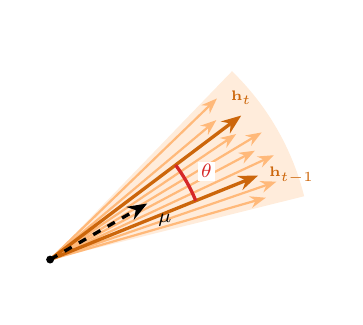
\begin{tikzpicture}[scale=0.95]
        \useasboundingbox (-0.3,-0.5) rectangle (3.8,3.1);
        \fill[machine!15] (0,0) -- (14:3.5) arc[start angle=14, end angle=46, radius=3.5] -- cycle;
        \foreach \a/\r in {16/3.0, 19/3.2, 25/3.3, 28/3.1, 31/3.3, 34/3.0, 40/2.9, 44/3.1}
          \draw[-{Stealth[length=2mm]}, machine!55, thick] (0,0) -- (\a:\r);
        \draw[-{Stealth[length=2.5mm]}, machine!80!black, very thick] (0,0) -- (22:3.0) node[right, font=\tiny] {$\mathbf h_{t-1}$};
        \draw[-{Stealth[length=2.5mm]}, machine!80!black, very thick] (0,0) -- (37:3.2) node[above, font=\tiny] {$\mathbf h_{t}$};
        \draw[-{Stealth[length=2.5mm]}, very thick, dashed] (0,0) -- (30:1.5) node[below right, font=\scriptsize] {$\mu$};
        \draw[very thick, bad] (22:2.1) arc[start angle=22, end angle=37, radius=2.1];
        \node[font=\scriptsize, text=bad, fill=white, inner sep=1pt] at (29.5:2.4) {$\theta$};
        \fill (0,0) circle (1.5pt);
      \end{tikzpicture}\\[2pt]
      {\scriptsize Token vectors cluster in a \textbf{narrow cone} around a shared direction $\mu$ and are
      \textbf{longer} $\Rightarrow$ \textbf{smaller} angles.}
    \end{column}
  \end{columns}
  \vspace{0.15cm}
  {\tiny Schematic of one early-to-middle layer: arrows are the hidden states of a text's tokens, $\mu$ is their centroid.}
  \vspace{0.1cm}
  \begin{takeaway}
    AI text fills a narrower cone, so any two of its tokens -- including neighbours -- are closer in angle.
  \end{takeaway}
\end{frame}

% ---------------------------------------------------------------
\begin{frame}{JAS \,|\, Analysis: Across-Layer -- Layers Rotate AI Tokens Less}
  \centering
  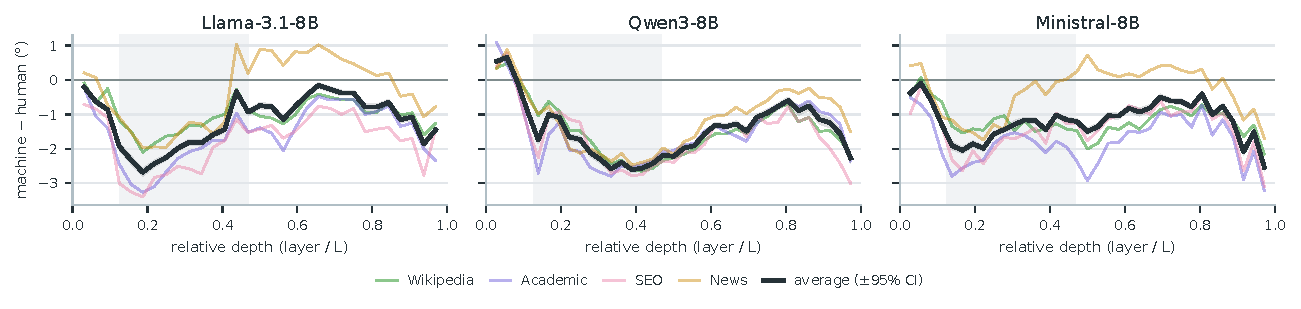
\includegraphics[width=\textwidth,height=3.65cm,keepaspectratio]{f_across_talk_A.pdf}\\
  {\tiny Angle of the same token between consecutive layers: machine $-$ human gap per layer, four DetectRL-X domains;
  grey band: layers 4--15.}
  \vspace{0.05cm}
  \raggedright\footnotesize
  \begin{itemize}\setlength{\itemsep}{1pt}
    \item In layers 4--15, layers rotate AI tokens \textbf{1.2--2.5$^\circ$ less} on average (up to 3.4$^\circ$),
          in \textbf{all four domains}.
    \item The gap is largest around \textbf{layers 5--7} and shrinks in the upper layers.
  \end{itemize}
  \begin{takeaway}
    Across layers, the hidden state of an AI token turns less from one layer to the next. \textbf{Why?}
  \end{takeaway}
\end{frame}

% ---------------------------------------------------------------
\begin{frame}{JAS \,|\, Analysis: Across-Layer -- Decomposing a Layer Update}
  \begin{columns}[c]
    \begin{column}{0.46\textwidth}
      \centering
      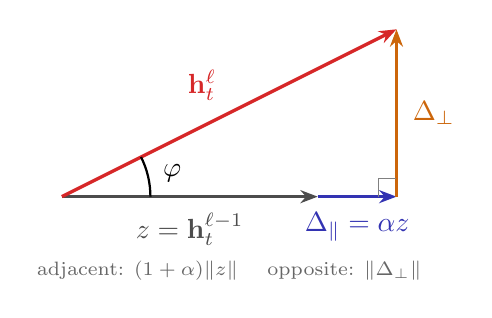
\begin{tikzpicture}[scale=1.25, >={Stealth[length=2.2mm]}]
        % z, its extension by alpha z, the perpendicular part and the new state
        \draw[->, very thick, black!70] (0,0) -- (2.6,0) node[midway, below=2pt] {$z=\mathbf h^{\ell-1}_t$};
        \draw[->, very thick, mainblue] (2.6,0) -- (3.4,0) node[midway, below=2pt] {$\Delta_\parallel=\alpha z$};
        \draw[->, very thick, machine!80!black] (3.4,0) -- (3.4,1.7) node[midway, right=2pt] {$\Delta_\perp$};
        \draw[->, very thick, bad] (0,0) -- (3.4,1.7) node[midway, above left=1pt] {$\mathbf h^{\ell}_t$};
        \draw[black!50] (3.22,0) -- (3.22,0.18) -- (3.4,0.18);
        \draw[thick] (0.9,0) arc[start angle=0, end angle=26.6, radius=0.9];
        \node at (1.12,0.24) {$\varphi$};
        \node[font=\scriptsize, black!60, align=center] at (1.7,-0.75)
          {adjacent: $(1+\alpha)\lVert z\rVert$ \quad opposite: $\lVert\Delta_\perp\rVert$};
      \end{tikzpicture}
    \end{column}
    \begin{column}{0.52\textwidth}
      \small
      Following \citet{he2026disentangling}, split each layer update $\Delta=\mathbf h^{\ell}_t-z$ along $z$:
      \[
        \alpha=\frac{\langle\Delta,z\rangle}{\lVert z\rVert^2},\qquad
        \Delta_\parallel=\alpha z,\qquad \Delta_\perp=\Delta-\alpha z
      \]
      \vspace{-2pt}
      \begin{itemize}\setlength{\itemsep}{1pt}
        \item \textcolor{mainblue}{$\Delta_\parallel$} \textbf{rescales} $z$ ($\alpha>0$ grows it, $\alpha<0$ shrinks it);
              \textcolor{machine!80!black}{$\Delta_\perp$} \textbf{turns} it ($\Delta_\perp\perp z$).
        \item So $\mathbf h^{\ell}_t=(1+\alpha)\,z+\Delta_\perp$: a right triangle, and
      \end{itemize}
      \[
        \tan\varphi=\frac{\text{opposite}}{\text{adjacent}}=\frac{\lVert\Delta_\perp\rVert}{(1+\alpha)\,\lVert z\rVert}
      \]
    \end{column}
  \end{columns}
  \vspace{2pt}
  \begin{takeaway}
    The angle is small when the state is large ($\lVert z\rVert$), grows along itself ($\alpha$), or gets a small
    sideways push ($\lVert\Delta_\perp\rVert$).
  \end{takeaway}
\end{frame}

% ---------------------------------------------------------------
\begin{frame}{JAS \,|\, Analysis: Across-Layer -- Why AI Tokens Rotate Less}
  \centering
  \vspace{-4pt}
  {\small $\displaystyle \tan\varphi=\frac{\lVert\Delta_\perp\rVert}{(1+\alpha)\,\lVert z\rVert}$,\quad
  $z=\mathbf h^{\ell-1}_t$,\; $\Delta=\mathbf h^{\ell}_t-z=\alpha z+\Delta_\perp$}\\[2pt]
  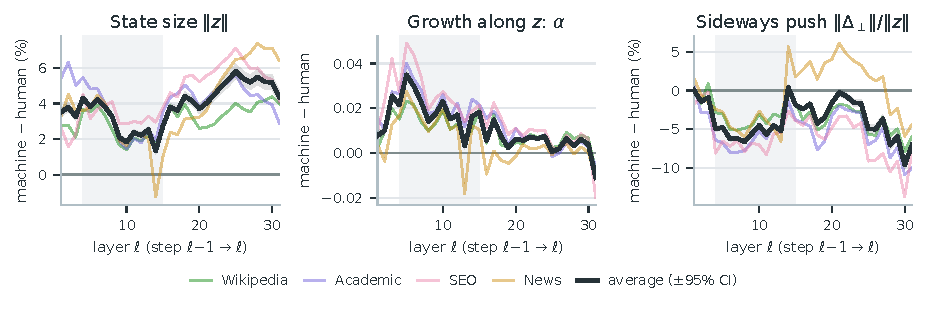
\includegraphics[width=\textwidth,height=3.4cm,keepaspectratio]{f_across_talk_B.pdf}\\
  {\tiny Machine $-$ human gap of each factor per layer; $\alpha$: update along $z$ ($<0$ shrinks $z$),
  $\Delta_\perp$: update at a right angle to $z$.}
  \vspace{0.05cm}
  \raggedright\footnotesize
  \begin{itemize}\setlength{\itemsep}{0pt}
    \item In layers 4--15, AI states are \textbf{larger} ($\lVert z\rVert$ +2.4--3.4\%), \textbf{shrink less}
          ($\alpha$ +0.013--0.027, on $\approx-0.065$) and get a \textbf{smaller sideways push}
          ($\lVert\Delta_\perp\rVert/\lVert z\rVert$ $-$3 to $-$6\%).
  \end{itemize}
  \begin{takeaway}
    \textbf{Finding 2:} layers rotate AI tokens less because three effects point the same way -- larger states,
    less shrinking and a smaller sideways push.
  \end{takeaway}
\end{frame}

% ---------------------------------------------------------------
\begin{frame}{JAS \,|\, Analysis: Not Just Predictability in Disguise}
  \centering
  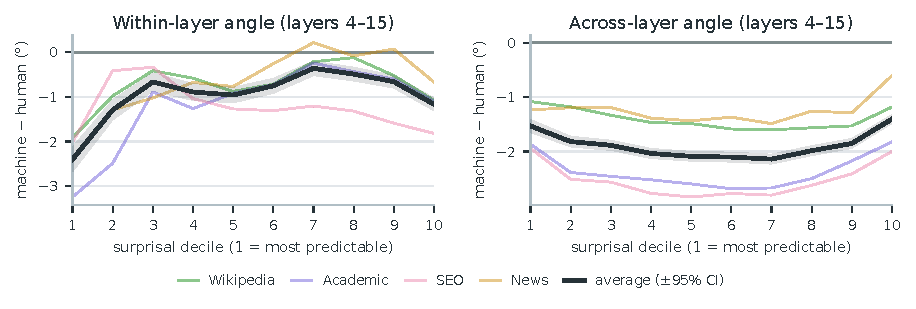
\includegraphics[width=\textwidth,height=3.65cm,keepaspectratio]{f_surprisal_talk.pdf}\\
  {\tiny Machine $-$ human angle gap for tokens of equal surprisal (deciles per domain), averaged over layers 4--15.}
  \vspace{0.05cm}
  \raggedright\footnotesize
  \begin{itemize}\setlength{\itemsep}{1pt}
    \item Many zero-shot detectors rely on token predictability, and AI text has more low-surprisal tokens.
    \item Comparing tokens \textbf{within the same surprisal decile}: the across-layer gap is negative in
          \textbf{every decile and domain} ($-$0.6 to $-$2.8$^\circ$); the within-layer gap in almost every one,
          largest for the most predictable tokens.
  \end{itemize}
  \begin{takeaway}
    The geometric signal captures human--AI differences that token surprisal does not explain.
  \end{takeaway}
\end{frame}

% ---------------------------------------------------------------
\begin{frame}{JAS \,|\, Analysis: Where in the Hidden State Is the Signal?}
  \centering
  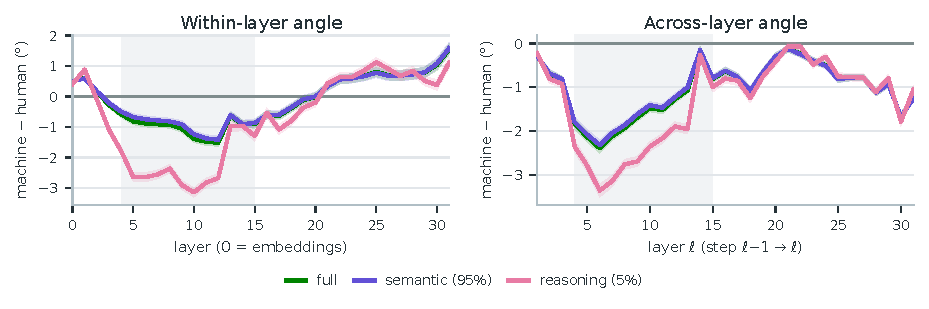
\includegraphics[width=\textwidth,height=3.65cm,keepaspectratio]{f_harp_talk.pdf}\\
  {\tiny Machine $-$ human angle gap per layer in each subspace, averaged over four DetectRL-X domains; grey band:
  layers 4--15.}
  \vspace{0.05cm}
  \raggedright\footnotesize
  \begin{itemize}\setlength{\itemsep}{1pt}
    \item \textbf{Subspaces:} an SVD of the unembedding $W_U$ ranks hidden directions by how strongly the output reads
          them; \textbf{semantic} = the top 95\%, \textbf{reasoning} = the bottom 5\% (205 of 4096 directions);
          states pass through the final norm first.
    \item \textbf{Results:} in layers 4--15 the gap is \textbf{largest in the reasoning subspace} -- within:
          $-$2.2$^\circ$ vs.\ $-$1.0$^\circ$ in the full space ($\sim$2$\times$); across: $-$2.2$^\circ$ vs.\ $-$1.5$^\circ$
          ($\sim$1.5$\times$) -- while semantic matches the full space.
  \end{itemize}
  \begin{takeaway}
    The human--AI difference is concentrated in a small subspace that the output layer barely reads.
  \end{takeaway}
\end{frame}

% ---------------------------------------------------------------
\begin{frame}{JAS \,|\, Methodology: The Joint Angular Score}
  \begin{columns}[c]
    \begin{column}{0.62\textwidth}
      \small
      Let $x=(x_1,\dots,x_n)$ be a text and $\mathbf h_t^{\ell}\in\mathbb R^d$ the hidden state of
      token $t$ at layer $\ell\in\{0,\dots,L\}$ of the scoring model ($\ell=0$: embeddings).
      Write $\angle(\mathbf a,\mathbf b)=\arccos\frac{\langle\mathbf a,\mathbf b\rangle}{\lVert\mathbf a\rVert\,\lVert\mathbf b\rVert}$.
      At each layer $\ell\ge 1$:
      \begin{align*}
        \theta_t^{\ell} &= \angle\big(\mathbf h_{t-1}^{\ell},\,\mathbf h_t^{\ell}\big)
          && \text{\scriptsize\textcolor{mainblue}{(within-layer: consecutive tokens)}}\\
        \varphi_t^{\ell} &= \angle\big(\mathbf h_t^{\ell-1},\,\mathbf h_t^{\ell}\big)
          && \text{\scriptsize\textcolor{machine!80!black}{(across-layer: consecutive layers)}}
      \end{align*}
      Per-token geometric mean of the two angles:
      \[
        J^{\ell}(x)=\frac{1}{|\mathcal T|}\sum_{t\in\mathcal T}\sqrt{\theta_t^{\ell}\,\varphi_t^{\ell}}
      \]
      \textbf{Detection score:} the joint angle $J^{\ell^*}(x)$ at layer $\ell^*$ --
      \textbf{lower} $\Rightarrow$ more likely AI-generated.
    \end{column}
    \begin{column}{0.35\textwidth}
      \centering
      \scalebox{0.7}{\trajschematic}
      \vspace{0.2cm}
      \begin{takeaway}
        The score follows directly from the analysis: AI tokens have smaller within- \emph{and}
        across-layer angles in early-to-middle layers.
      \end{takeaway}
      \vspace{0.1cm}
      {\scriptsize Zero-shot: no training data, one forward pass of the scoring model.}
    \end{column}
  \end{columns}
\end{frame}

% ---------------------------------------------------------------
\begin{frame}{JAS \,|\, Result 1: Detection Across Domains}
  \centering
  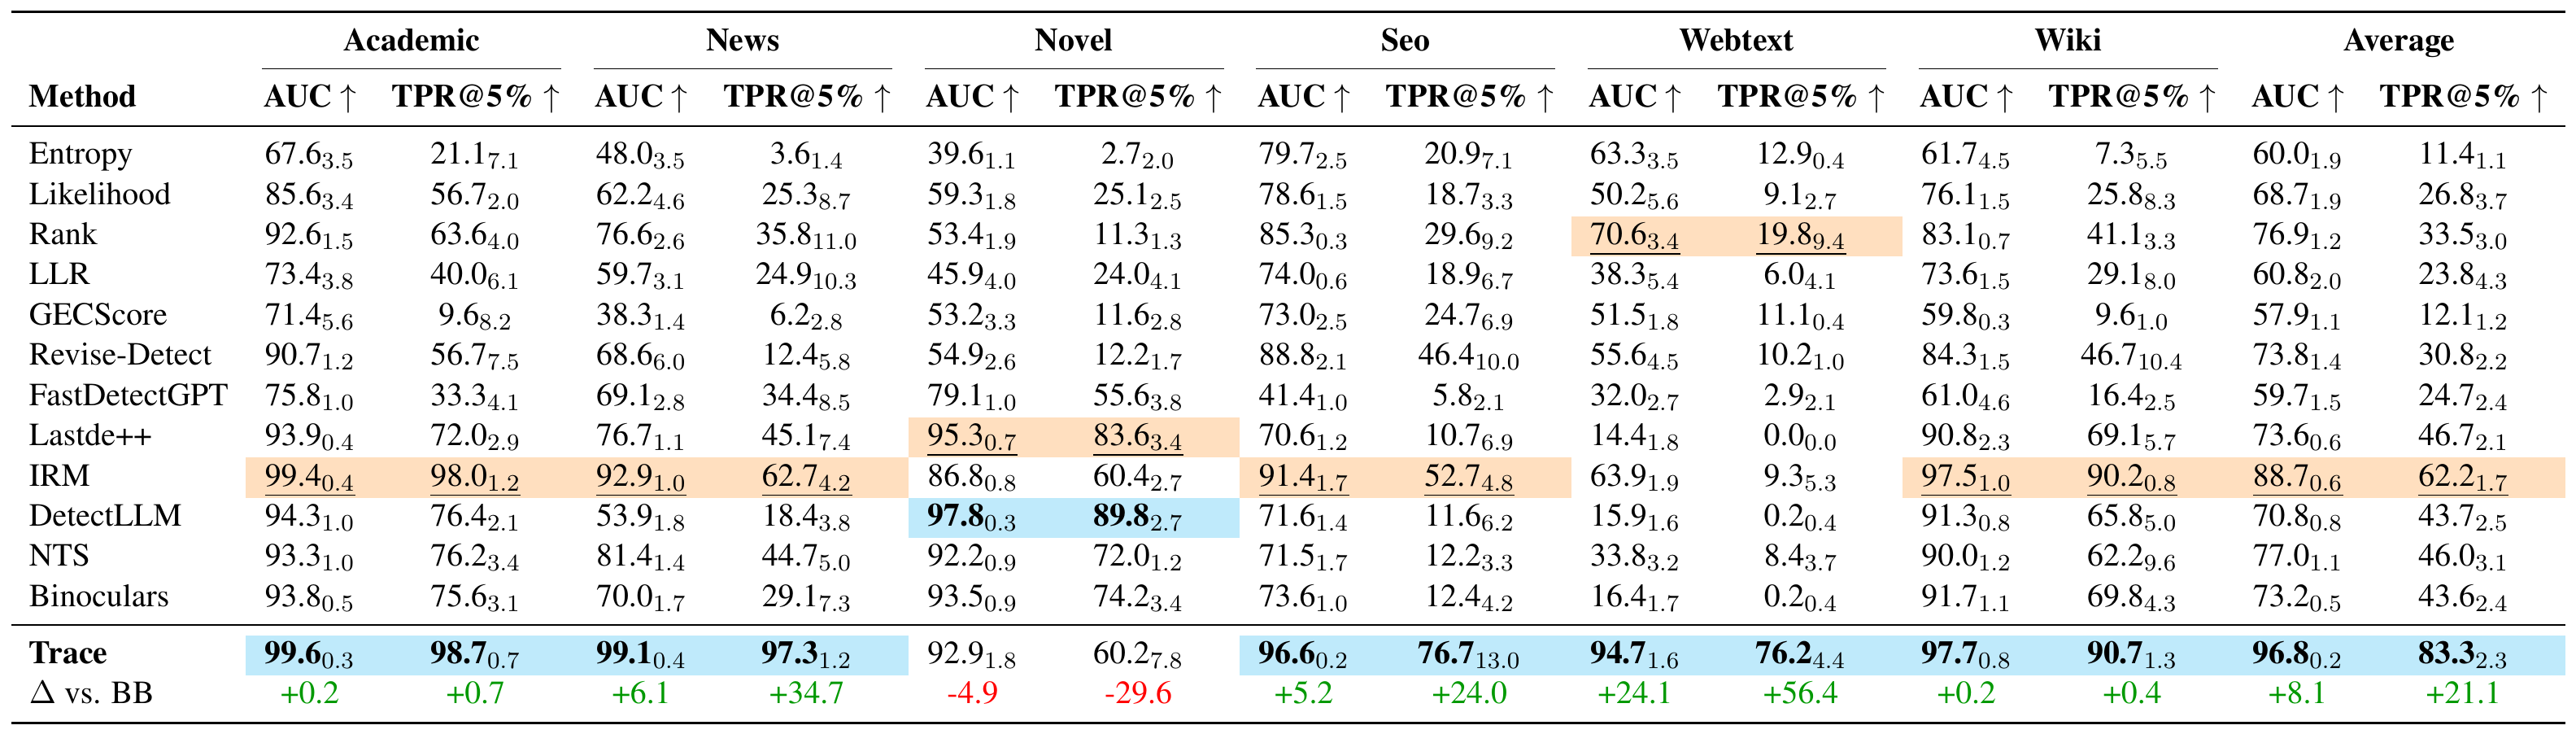
\includegraphics[width=0.9\textwidth]{z_tab1.png}\\
  {\tiny Domain subset of DetectRL-X: AUC and TPR at 5\% FPR (mean$_{\text{std}}$) against 12 zero-shot detectors.}
  \vspace{0.15cm}
  \raggedright\small
  \begin{itemize}
    \item Best average AUC (\textbf{96.8} vs.\ 88.7 for IRM) and TPR@5\% (\textbf{83.3}, +21.1).
    \item Largest gain on Webtext (+24.1 AUC), where most detectors collapse; only on Novel is JAS
          below the best baseline ($-$4.9).
  \end{itemize}
  \begin{takeaway}
    JAS is the strongest zero-shot detector across domains -- especially at low false-positive rates.
  \end{takeaway}
\end{frame}

% ---------------------------------------------------------------
\begin{frame}{JAS \,|\, Result 2: Detection Across Generators}
  \centering
  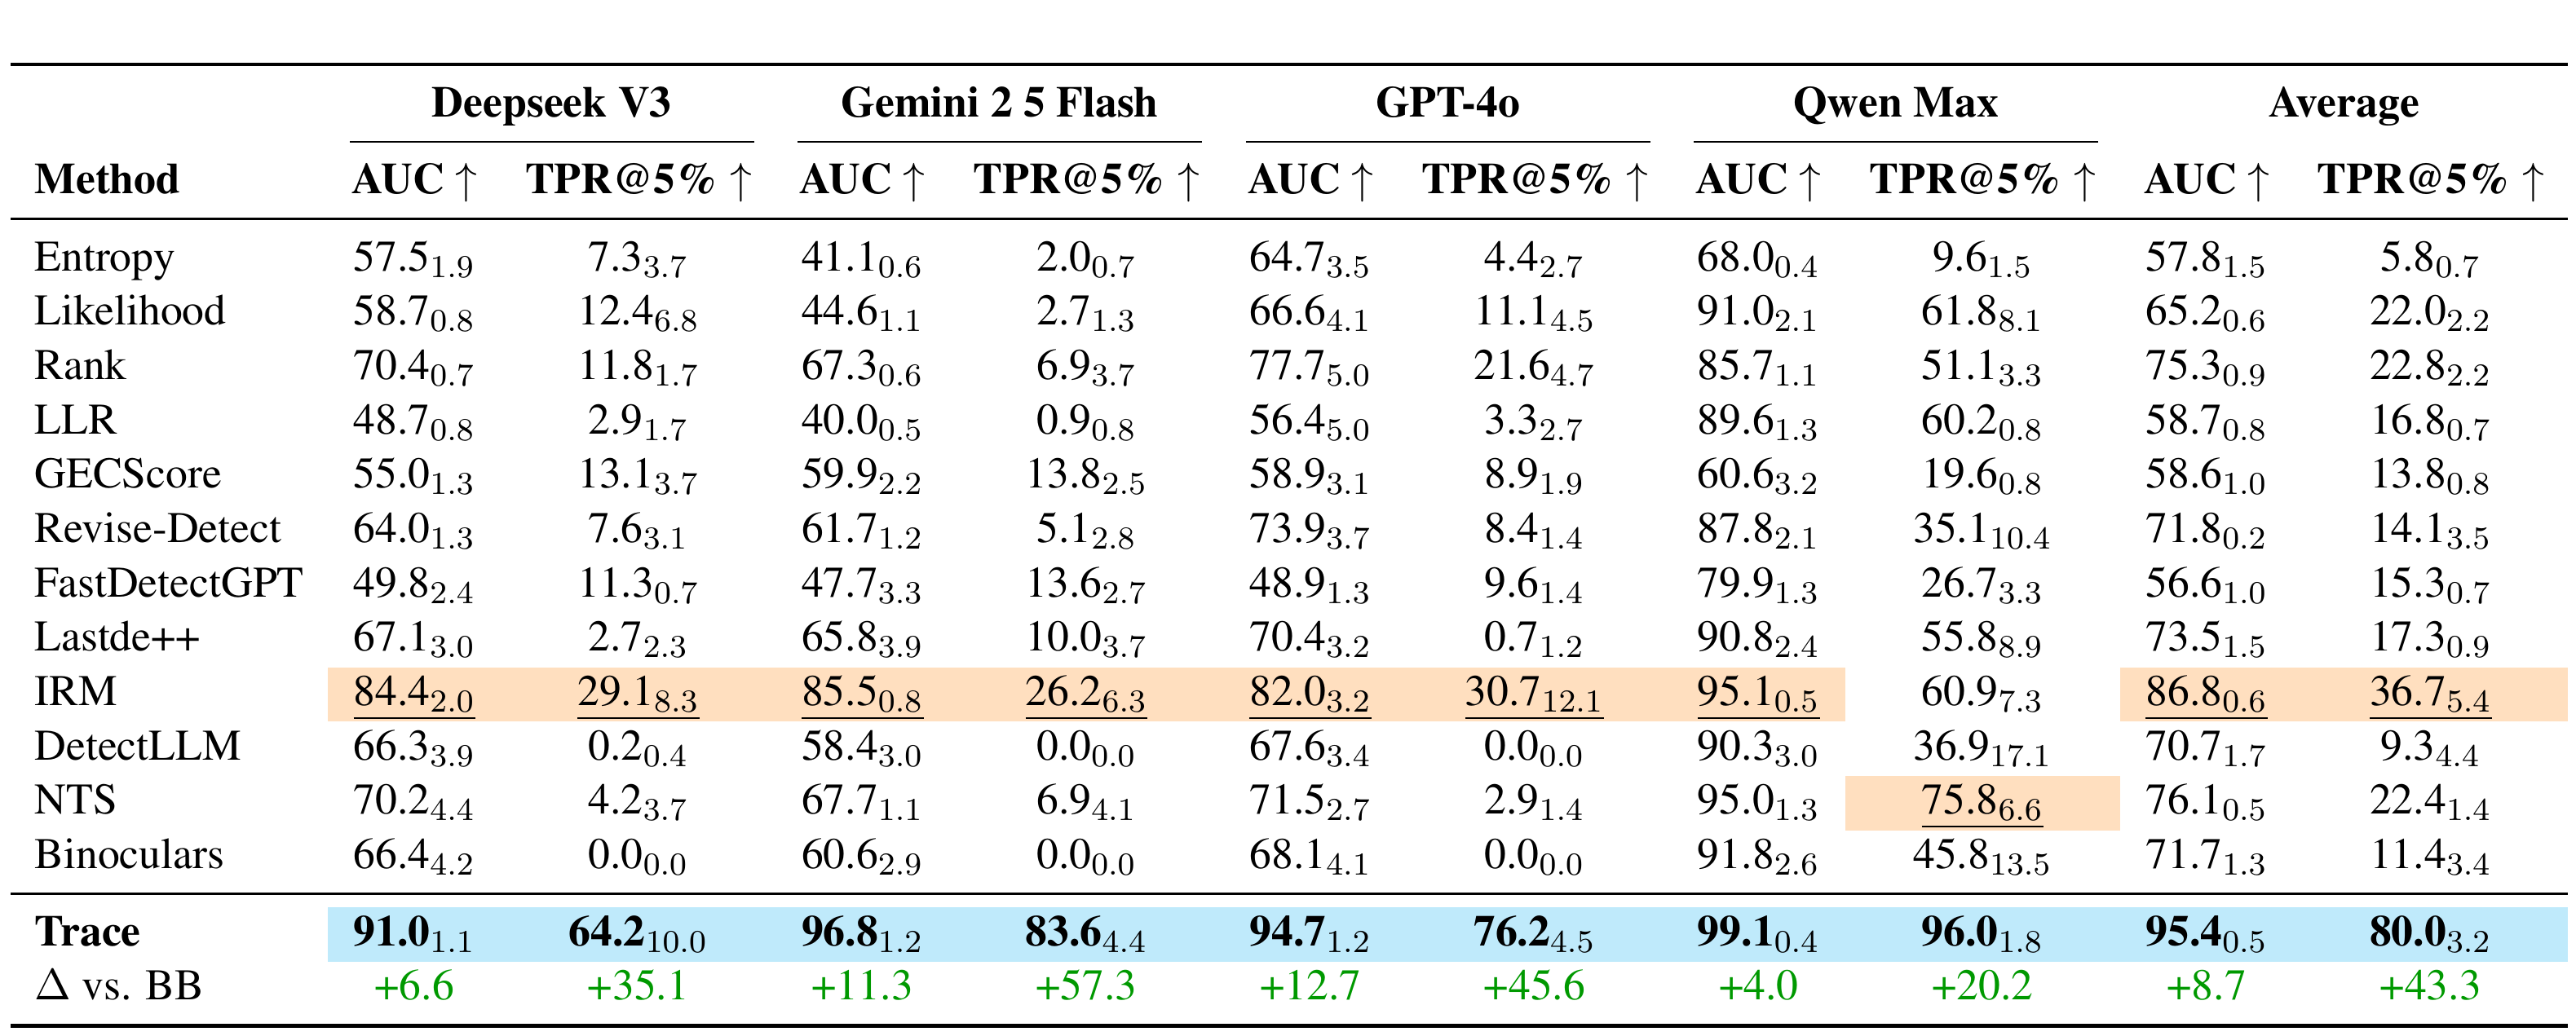
\includegraphics[width=0.68\textwidth]{z_tab2.png}\\
  {\tiny Generator subset of DetectRL-X: AUC and TPR at 5\% FPR against 12 zero-shot detectors.}
  \vspace{0.1cm}
  \raggedright\footnotesize
  \begin{itemize}
    \item Best on \textbf{all four} generators: average AUC \textbf{95.4} (+8.7) and TPR@5\% \textbf{80.0} (+43.3).
    \item Largest gain on Gemini 2.5 Flash (+11.3 AUC, +57.3 TPR@5\%), where most baselines barely detect anything at low FPR.
  \end{itemize}
  \begin{takeaway}
    JAS detects text from frontier generators far more reliably than existing zero-shot detectors.
  \end{takeaway}
\end{frame}

% ---------------------------------------------------------------
\begin{frame}{JAS \,|\, Result 3: Robustness to Evasion Attacks}
  \centering
  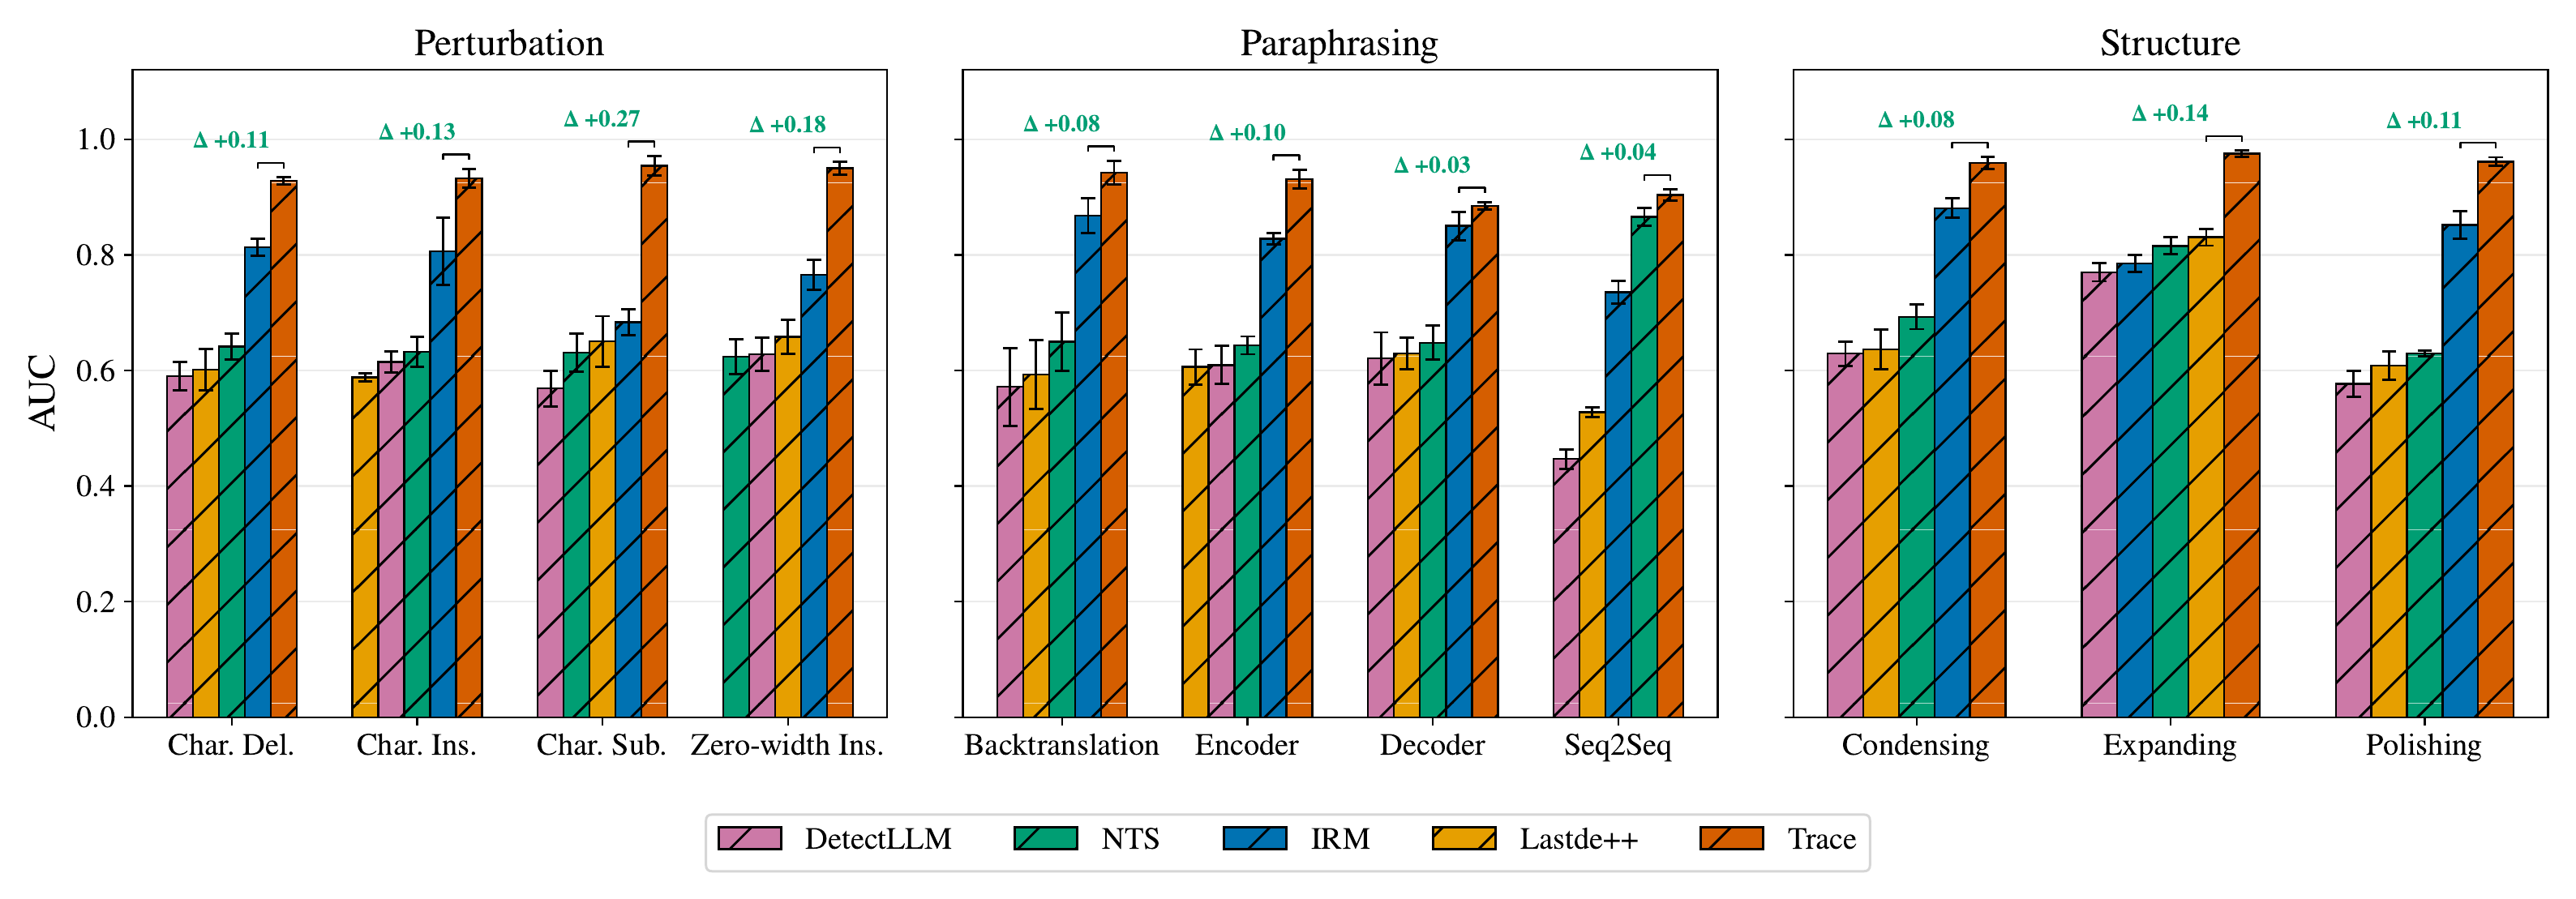
\includegraphics[width=0.8\textwidth]{z_fig8.png}\\
  {\tiny AUC under 11 evasion attacks; $\Delta$ = gain over the strongest baseline.}
  \vspace{0.15cm}
  \raggedright\small
  \begin{itemize}
    \item Three attack families: character perturbations, paraphrasing and structural rewrites.
    \item JAS wins in every setting (+0.03 to +0.27 AUC), most clearly under character substitution.
  \end{itemize}
  \begin{takeaway}
    JAS remains the best detector under all 11 evasion attacks.
  \end{takeaway}
\end{frame}

% ---------------------------------------------------------------
\begin{frame}{JAS \,|\, Result 4: Short Texts}
  \begin{columns}[c]
    \begin{column}{0.50\textwidth}
      \centering
      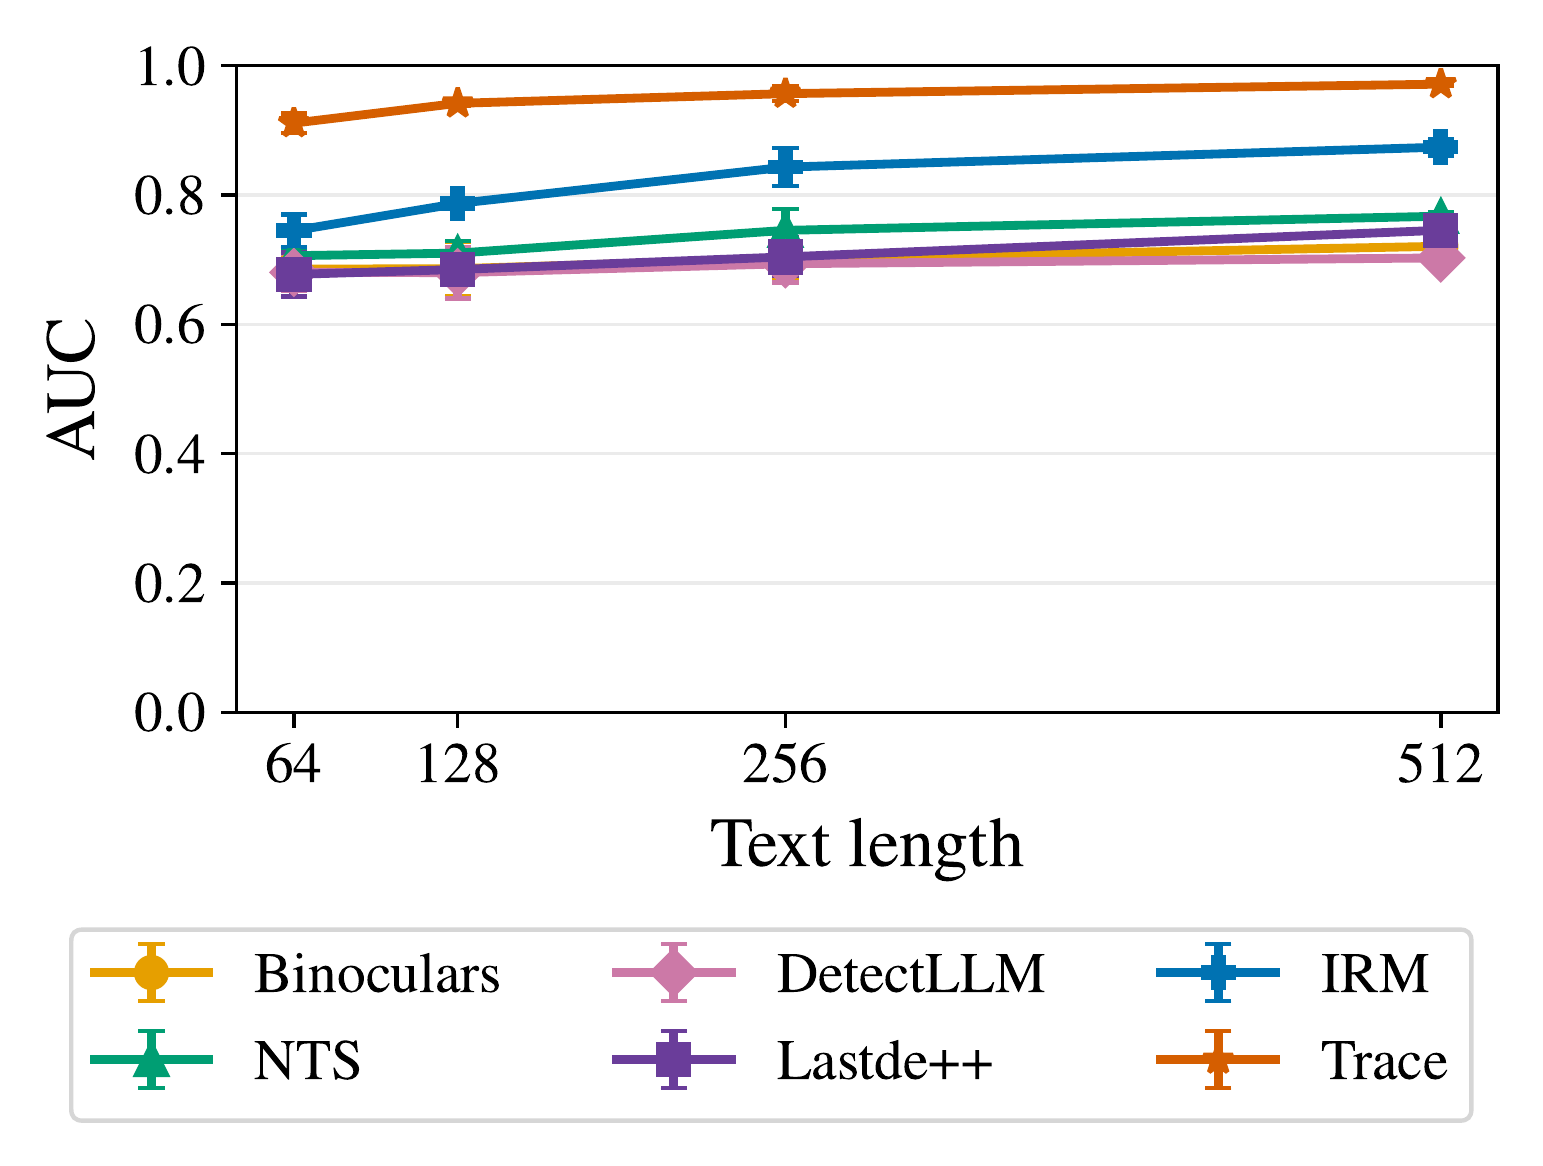
\includegraphics[width=0.95\textwidth]{z_fig9.png}\\
      {\tiny AUC as a function of text length (tokens).}
    \end{column}
    \begin{column}{0.47\textwidth}
      \begin{itemize}
        \item JAS reaches $\sim$0.91 AUC with only \textbf{64 tokens}, rising to $\sim$0.97 at 512.
        \item Best detector at \textbf{every length}; the runner-up (IRM) goes from $\sim$0.75 to $\sim$0.87.
      \end{itemize}
      \vspace{0.2cm}
      \begin{takeaway}
        JAS stays reliable even on short texts.
      \end{takeaway}
    \end{column}
  \end{columns}
\end{frame}

% ---------------------------------------------------------------
\begin{frame}{JAS \,|\, Result 5: Speed and Memory}
  \centering
  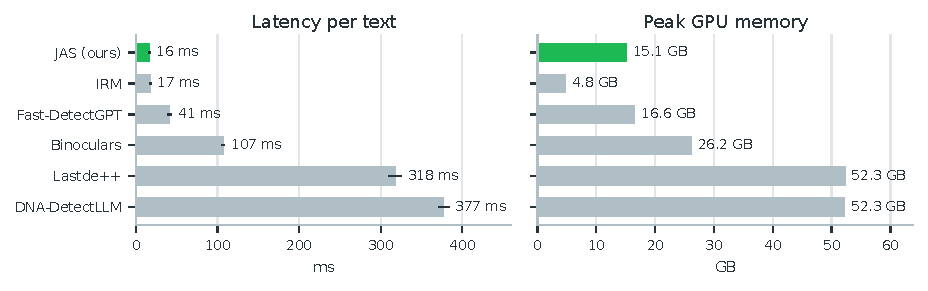
\includegraphics[width=\textwidth,height=3.55cm,keepaspectratio]{f_time_space_talk.pdf}\\
  {\tiny Per text at batch size 1 on one NVIDIA H200 (300 Wikipedia texts); latency: mean $\pm$ std; memory: peak
  allocated, weights included.}
  \vspace{0.05cm}
  \raggedright\footnotesize
  \begin{itemize}\setlength{\itemsep}{1pt}
    \item \textbf{Fastest}, on par with IRM: 16\,ms per text -- one forward pass of one model; 6.6$\times$ faster
          than Binoculars and $\sim$20$\times$ faster than Lastde++ and DNA-DetectLLM.
    \item \textbf{Memory:} 15\,GB for one 8B model, below the two-model detectors (17--52\,GB); only IRM (two 1B models)
          needs less.
  \end{itemize}
  \begin{takeaway}
    JAS is cheap to run: no training, no second model, one forward pass per text.
  \end{takeaway}
\end{frame}

% ---------------------------------------------------------------
\begin{frame}{JAS \,|\, Result 6: Token-Level Interpretability}
  \centering
  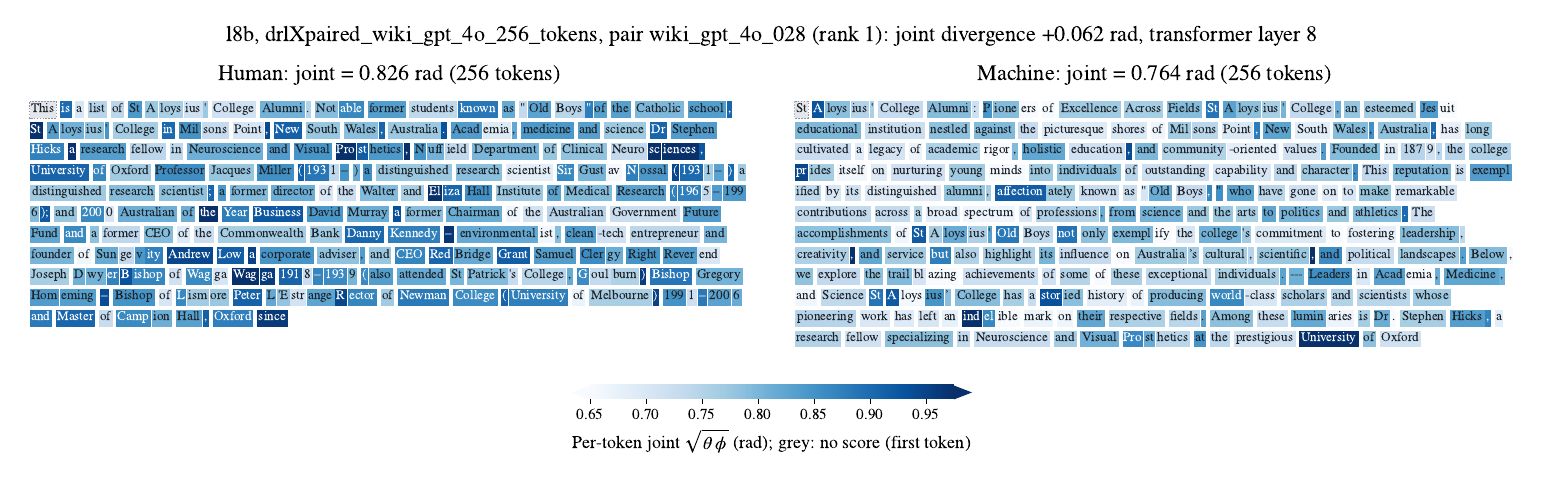
\includegraphics[width=0.8\textwidth]{z_fig10.png}\\
  {\tiny Per-token joint angle $\sqrt{\theta\varphi}$ at layer 8 for a human (left) and an AI-generated (right) Wikipedia text (GPT-4o).}
  \vspace{0.1cm}
  \raggedright\small
  \begin{itemize}
    \item Every token gets its own joint angle, so the score can be shown \textbf{directly on the text}.
    \item Lower angles flag \textbf{``AI style''}, e.g.\ purple prose such as \emph{``picturesque shores''} or \emph{``outstanding capability and character''}.
  \end{itemize}
  \begin{takeaway}
    Token-level angles show \emph{where} a text looks machine-generated, not just \emph{whether}.
  \end{takeaway}
\end{frame}

% ---------------------------------------------------------------
\begin{frame}{JAS \,|\, Main Takeaways}
  \small
  \renewcommand{\arraystretch}{1.5}
  \begin{tabular}{@{}>{\raggedright\arraybackslash}p{0.45\textwidth} >{\raggedright\arraybackslash}p{0.50\textwidth}@{}}
    \toprule
    \textbf{Takeaway} & \textbf{Why it matters for} \spotifylogo \\
    \midrule
    \textbf{1. AI text leaves a geometric fingerprint.}
    In early-to-middle layers, AI tokens are more aligned and rotate less -- beyond what
    perplexity explains.
    & A signal beyond perplexity helps on content that is predictable by nature (templated
      descriptions, metadata), where likelihood-based detectors may misfire. \\
    \textbf{2. A training-free score beats 12 zero-shot detectors}
    (+8 AUC; +21 to +43 TPR at 5\% FPR).
    & No labelled data needed: usable on new surfaces, languages and generators right away; strong
      detection at low false-positive rates matters when wrongly flagging creators is costly. \\
    \textbf{3. Robust and interpretable.} Best under 11 evasion attacks and on texts of 64 tokens,
    with token-level explanations.
    & Fits short-form text (titles, descriptions, comments) and gives reviewers token-level
      evidence for moderation decisions. \\
    \bottomrule
  \end{tabular}
\end{frame}

% ---------------------------------------------------------------
\againframe{glance}

% ---------------------------------------------------------------
\begin{frame}{Future Questions}
  \begin{itemize}\setlength{\itemsep}{10pt}
    \item How can we use linear probes for \textbf{fine-grained} (span- or token-level) detection?
          $\Rightarrow$ \textbf{attention probes}
    \item How does the \textbf{latent AI direction} influence text generation and text representations?
    \item Does the idea of a latent AI direction hold \textbf{across modalities}?
    \item How can we build a benchmark that separates \textbf{human ideation} from \textbf{AI writing}?
    \item How do text representations differ in models trained \textbf{only on machine-generated}
          vs.\ \textbf{only on human-written} text?
  \end{itemize}
\end{frame}

% ===============================================================
\begin{frame}{References}
  \footnotesize
  \bibliographystyle{plainnat}
  \bibliography{references}
\end{frame}

% ===============================================================
\begin{frame}
  \centering
  {\Huge Thank you!}\\[0.6cm]
  {\Large Questions?}\\[1cm]
  \small
  TSM-Bench: \texttt{github.com/gerritq/tsm\_bench}\\[2pt]
  \texttt{gerrit.quaremba@kcl.ac.uk}
\end{frame}

\end{document}
